\documentclass[a4paper]{article}
% Options possibles : 10pt, 11pt, 12pt (taille de la fonte)
% oneside, twoside (recto simple, recto-verso)
% draft, final (stade de développement)
\usepackage[utf8]{inputenc}   % LaTeX, comprends les accents !
\usepackage[T1]{fontenc}      % Police contenant les caractères français
\usepackage[french]{babel}
\usepackage{fullpage}
%\usepackage{xcolor}
\usepackage{hyperref} %pour les liens
\usepackage{float}
\usepackage[dvipsnames]{xcolor}
\usepackage{amsmath}
\usepackage{pgfgantt}
\usepackage{easyReview}
\newcommand{\axel}[1]{{\color{violet} #1 }}
\newcommand{\satine}[1]{{\color{WildStrawberry} #1 }}
\newcommand{\sauranne}[1]{{\color{blue} #1 }}
\newcommand{\gaelle}[1]{{\color{olive} #1 }}
\usepackage{graphicx}  % pour inclure des images
%\pagestyle{headings}        % Pour mettre des entêtes avec les titres               % des sections en haut de page
\title{Simulation de fluides en 2D \\ % Les paramètres du titre : titre, auteur, date
Projet de programmation 2}
\author{Axel Pereyrol, Saurane Delrieu, Gaelle Milezi, Satine Barraux \\
    \emph{L3 informatique} \\
    Faculté des Sciences \\
    Université de Montpellier
}
\date{2025-2026}
\begin{document}


\maketitle     % Faire un titre utilisant les données               % passées à \title, \author et \date
%\begin{center}               % pour centrer
% \includegraphics[scale=1]{}   % insertion d'une image
%\end{center}
\begin{abstract}     % Résumé du travail
Ce projet de simulation de fluides en 2D consiste à rendre de manière interactive et 
en temps réel l'évolution d'un fluide dans une grille. Nous avons implémenté la 
méthode de Jos Stam "Stable Fluids" \cite{Stam99} pour simuler le fluide, et nous 
avons développé une interface graphique pour visualiser et interagir avec la 
simulation. L'utilisateur peut ajouter des sources de fluide, créer des obstacles, et 
modifier les paramètres du fluide en temps réel. 
\end{abstract}
\newpage
%\dominitoc  % initializer les minitoc
\tableofcontents
\newpage

\section{Présentation du Sujet} % Commencer une section, * permet de ne pas numéroté l'introduction
\remove{\emph{1-2 pages}}
%Présentation du Sujet (1-2 pages)
% \begin{itemize}%pour faire une liste à puces
%1.1		SATINE
\remove{Présenter le problème étudier et le contexte dans lequel le projet se positionne.}

\satine{
    Ce projet de programmation 2 a été réalisé dans le cadre de la licence informatique L3  de la faculté des sciences de Montpellier. L'objectif de ce projet est de simuler un fluide de manière interactive en 2D en temps réel. Pour cela, nous avons choisi d'implémenter la méthode de Jos Stam "Stable Fluids" \cite{Stam99}, qui permet de simuler un fluide de manière stable et rapide. Nous avons également implémenté une interface graphique pour  visualiser en temps réel l'évolution du fluide et pour intéragir avec celui-ci. Cette intéraction est possible grâce à la création  d'obstacles clicables et la possibilité de modifier durant la simulation les différents paramètres du fluide.
}

%1.2		SAURANE
\remove{Motiver l'intérêt du problème étudié par rapport à votre parcours d'études et au monde de l'informatique.}

\sauranne {
    \replace{Nous avons choisi ce projet car il nous a paru être le plus adapté à nos compétences, étant donné notre parcours en double licence mathématiques et informatique}{Étant donné notre parcours en double licence mathématique et informatique, ce projet est bien adapté à nos compétences}. En effet, nous avons \add{pu} rapidement comprendre les concepts de base de la simulation, ce qui nous a permis d'implémenter la méthode de Jos Stam "Stable Fluids" \cite{Stam99}.

\replace{Nous avons également aimé l'idée d'implémenter une interface graphique pour observer l'évolution du fluide}{L'implémentation d'une interface graphique pour interagir avec le fluide et observer son comportement nous a fortement intéressé}. \comment{}{La forme passive est préférable, je trouve} De plus, \replace{c'est avec ce projet que}{au travers ce projet,} nous avons découvert le langage C++ et la bibliothèque OpenGL, qui sont des outils essentiels dans \add{de nombreux domaines tels que} la simulation de fluides\remove{mais aussi dans de nombreux domaines tels que}, les jeux vidéos, la météorologie ou l'environnement.
}

%1.3	    SAURANE
\remove{Présenter les différentes approches possibles pour la résolution du problème, et en particulier celle choisie.}

\sauranne {
    \replace{Pour implémenter la simulation de fluides en 2D, deux méthodes sont possibles}{Principalement trois familles de méthodes existent pour implémenter une simulation de fluide} : les méthodes eulériennes, les méthodes lagrangiennes \add{, et les méthodes semi-lagrangiennes, qui sont des hybrides des deux précédentes}. Les méthodes eulériennes consistent à représenter le fluide dans une grille \remove{fixe}, où l'on stocke les différentes propriétés du fluide, telles que la densité, la chaleur, la vitesse, etc. \add{Chaque cellule represente une portion du fluide, encodant les propriétés du fluide dans une région en un instant $t$.}

Les méthodes lagrangiennes consistent, quant à elles, à représenter le fluide à l'aide de \add{nombreuses} particules, \replace{c'est à dire que chaque particule contient les propriétés du fluide}{représentant les gouttes ou molécules du fluides. L'ensemble de ces particules déterminent les propriétés du fluide}.
}

\sauranne {
    Pour l'implémentation de ce projet, nous avons choisi la méthode eulérienne, qui est plus simple à implémenter et moins coûteuse en complexité. La méthode lagrangienne peut rapidement exploser en temps de calcul en fonction du nombre de particules.
    \comment{}{Pourquoi le lagrangien est plus coûteux ? Décrire que les interactions entre toutes les particules tendent à une complexité en $\mathcal{O}(n^2)$ (n = nombre de particules) contre $\mathcal{O}(n)$ (n = nombre de cellules) en eulerien. }
}

%1.4           GAËLLE
\remove{Donner le cahier des charges détaillé}

\gaelle {
    Le cahier des charges du projet, réalisé en décembre 2025, fixait le cadre de développement, et définissait les objectifs, les contraintes et les fonctionnalités (minimales) à implémenter. Vous trouverez à la suite une synthése de celui-ci.
\begin{itemize}
        \item Le projet consistait à développer un rendu interactif permettant la visualisation et la manipulation en temps réel d'une simulation de fluide en 2D. Comme précisé lors de la réunion avec notre responsable de projet, la simulation devait être interactive et comporter une interface graphique. Nous avions fait le choix de développer ce projet en C++ avec un affichage en OpenGL.
        \item L'objectif principal était d'obtenir une zone de rendu avec, d'un coté la simulation, et de l'autre une fenêtre de gestion des paramètres. Lors de la première réunion nous avions également déterminé le périmètre du projet. Nous avions décidé que la simulation reposerait sur une approche Eulerienne du fluide dans une grille 2D de taille $100 \times 100$.
        \item Nous avions également pensé aux fonctionnalités que nous pourrions rajouter comme la connexion bluetooth à un téléphone permettant de gérer la simulation ou encore l'ajout de musique en fonction des forces du fluide. Enfin, nous avions imaginé une organisation modulaire (calcul du fluide, interactions, affichage), permettant une répartition optimale des tâches \add{et un découpage plus propre de notre code}. 
\end{itemize}
}
% \end{itemize}




\section{Développements Logiciel : Conception, Modélisation, Implémentation}
\remove{\emph{8 à 15 pages}}
% \begin{enumerate} %pour faire une liste numérotée
%2.1         AXEL
\subsection{Technologies utilisées}
\begin{itemize}
        \item langage de programmation : C++ (justification pour l'optimsation, etc)
        \item openGL (affichage : api graphique)
        \item Imgui (facile d'utilisation)
\end{itemize}

%============================== AXEL 1 =======================================
\axel{
    \comment{}{Ça, ça devait changer..!}
    Pour notre projet, nous hésitions entre du C++ et du Python ; nous avons opté pour du C++ pour un typage plus fort et une meilleure gestion de ce qu'il se passe en mémoire et en interne plus généralement.
    \comment{}{"De nombreux langages de programmation existent, néanmoins nous nous sommes orientés sur le langage C++ : en plus de proposer une importante puissance de calcul nécessaire pour la simulation de fluide, ce langage fortement typé nous oblige à collaborer avec plus de rigueur, ... bla bla bla ... "}

\replace{À partir de la nous avions deux options concernant l'API graphique : SFML et OpenGL}{Il existe plusieurs API graphiques pour l'affichage à l'écran, notamment OpenGL, Vulkan, SDL, SFML, etc}. Nous avons ici choisi OpenGL afin de pouvoir déléguer au GPU et parce que nous avions déjà quelques bases dans le langage (grâce à l'excellent cours Learn OpenGL de Joey De Vries \add{\cite{LearnOpenGL}}).

\remove{Une fois en C++ sur OpenGL,} nous avons établi des prémices d'interactivité via le terminal, avant de basculer sur IMGUI \replace{(voir le Github polyvalent de Ocornut)}{\cite{ImGUI}}, qui s'impose comme une référence en terme de panneau de contrôle interactif en OpenGL.
}

%=============================================================================
%2.2      GAËLLE
\remove{Présenter les développements logiciel réalisés dans le cadre du projet. (fenetre, zone de rendu et panneau de parametres, et zone de rendu (shader, openGL))}
\subsection{Développements logiciel réalisés}
\gaelle {
    Dans cette partie nous allons nous intéresser à l'architecture de notre projet.
    
Le diagramme UML (\replace{voir figure5}{Figure~\ref{diagUML}}) suivant décrit \add{brièvement} l'organisation du projet \add{que nous décrirons en détails par la suite}. Nous pouvons clairement distinguer les principaux modules :
\begin{itemize}
        \item Données : module qui regroupe les structures représentant la grille, les cellules et les particules (nous
    vons également inclu la classe Simulation pour des raisons de clarté);
        \item Fluid Solver : qui implémente les étapes de la simulation ;
        \item Zone de rendu : ce module permet l'affichage en OpenGL ;
        \item Fenêtre de paramètres : interface Imgui  ;
        \item Interaction utilisateur : ce module traite les actions du clavier ou de la souris ;
        \item Gestion des obstacles : il a pour but de réunir ce qui touche aux obstacles, la création et le déplacement de ceux-ci.
\end{itemize}

\begin{figure}[H]
    \centering
    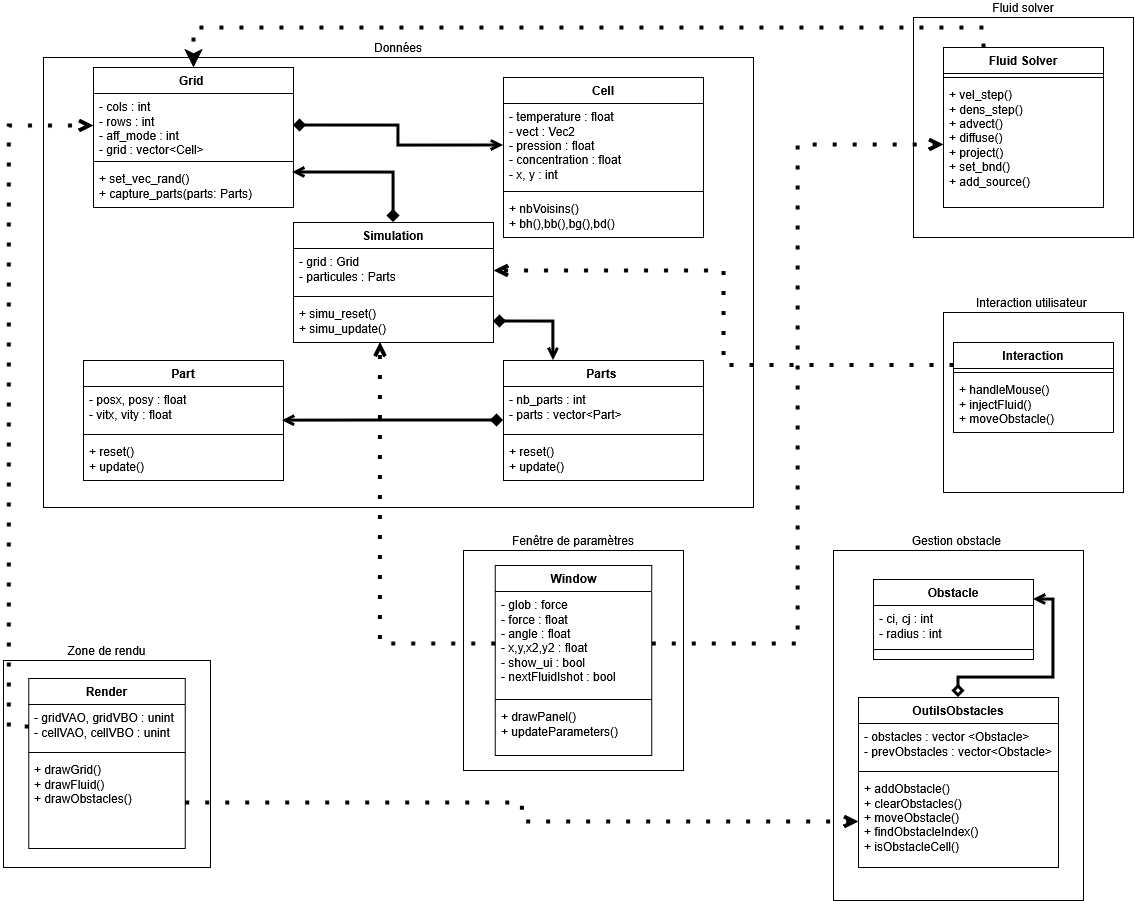
\includegraphics[width=0.9\textwidth]{../PJ_proj/diag_uml.drawio.png}
    \caption{Diagramme UML \add{de notre projet. Les flèches indiquent ..., les pointillés décrivent ... }}
    \label{diagUML}
\end{figure}

Ce diagramme permet de visualiser les dépendances entre modules et la structure de la simulation.
}

\gaelle {
    Nous allons maintenant présenter les différents composants de l'affichage et de l'interface de notre projet. L'interface finale repose sur plusieurs éléments, l'affichage d'une grille de chaleur, la visualisation du fluide, un panneau de paramètres et la gestion des obstacles. Ces composants constituens l'ensemble des fonctionnalités mis en oeuvre durant le projet.
}

\subsubsection{Affichage d'une grille de chaleur}
\comment{}{Les références aux figures doivent être dans le texte, pas dans les titres.}
\gaelle {
    Nous avons mis en place un affichage sous forme de grille de chaleur \add{(Figure~\ref{figure1})}. Pour mettre en place cet affichage, chaque cellule de la grille est associée à une valeur (dans \replace{notre}{ce} cas, cette valeur représente une température). Nous utlisons différentes teintes de rouge afin de représenter visuellement les variations de température : une cellule très chaude apparaît plus rouge, tandis qu'une cellule voisine un peu moins chaude aura une teinte moins rouge. Cet affichage permet de visualiser \replace{(de manière plutôt intuitive)}{intuitivement} l'évolution d'un champ scalaire.

    \comment{}{Évitez le texte entre parenthèse. Les parenthèses servent à décrire quelque chose qui n'est pas si important dans un texte. Par exemple "(reset, update, etc.)" qu'on retrouve 2 paragraphes plus bas.}

    \comment{}{Comment la chaleur évolue ? "Diffusion", "mélange avec ses voisins", etc.}
}

\begin{figure}[H]
    \centering
    
\includegraphics[width=0.45\textwidth]{../PJ_proj/carte_chaleur.png}
    \caption{Affichage d'une grille de chaleur. \add{Le rouge représente ... le bleu représente ... La température dans la région centrale s'uniformise plus vite que les bords ...} \comment{}{Si vous avez 2 images avant/après, ça permet de voir une évolution. Une seule, c'est pas vraiment une évolution}}
    \label{figure1}
\end{figure}

\axel{
    Nous avons une simulation de fluide Eulérienne, qui fonctionne sur le principe d'une grille dont chaque cellule possède ses paramètres locaux. Nous avons donc implémenté notre grille avec un simple \add{std::}vecteur C++ de structure Cell avec chaque paramètre comme attribut.

    \comment{}{std::vector = tableau unidimensionnel (1D) -> car plus rapide sur le CPU pour faire des calculs.}

    \comment{}{Ajouter une image du diagramme UML avec seulement "Simulation", "Grid" et "Cell", puis la référencer dans le texte.}

\comment{Cette grille possède ses propres méthodes (reset, update, \emph{etc...}). Nous l'avons définie à la base de notre arborescence d'inclusion de fichiers afin d'en faire un Singleton : structure unique de référence accessible depuis n'importe quel module du projet.}{Attention, ce n'est pas le cas dans votre diagramme UMl. Vous pouvez dire que vous l'avez divisée en deux parties : "Grid" et "Simulation".}
}

\subsubsection{Simulation du fluide (voir Figure~\ref{figure2})}
\comment{}{Déplacer la référence à l'image et la placer dans le texte}

\comment{}{Section à merger avec celle au-dessus ? }
\gaelle {
    La simulation du fluide repose sur la méthode Jos Stam \emph{Real-Time Fluid Dynamics for Games} \add{\cite{Stam03}} qui nous a permit d'avoir un \replace{beau rendu}{rendu dynamique} en 2D. Le fluide est représenté sur une grille Eulerienne 
    (voir section \comment{....}{Pour se référer à une section, vous pouvez ajouter un '$\backslash$label$\{$sec:nom-de-la-section$\}$' sous une $\backslash$section ou $\backslash$subsection|, puis s'y référer avec "Section$\sim\backslash$ref$\{$sec:nom-de-la-section$\}$". Par exemple : "Section~\ref{sec:interface-utilisateur}"}). 
    Dans cette grille, chaque cellule stocke des informations phyiques comme la densité ou la vitesse \add{sous forme de scalaire (\texttt{float}) ou de vecteur (paire de \texttt{float})}. A chaque itération de la simulation, ces données sont mis à jour grâce aux méthodes physiques comme l'advection, la diffusion ou la projection \add{que nous présenterons en détails dans la partie ...}. La zone de rendu affiche donc la densité du fluide en temps réel.
}

\begin{figure}[H]
    \centering
    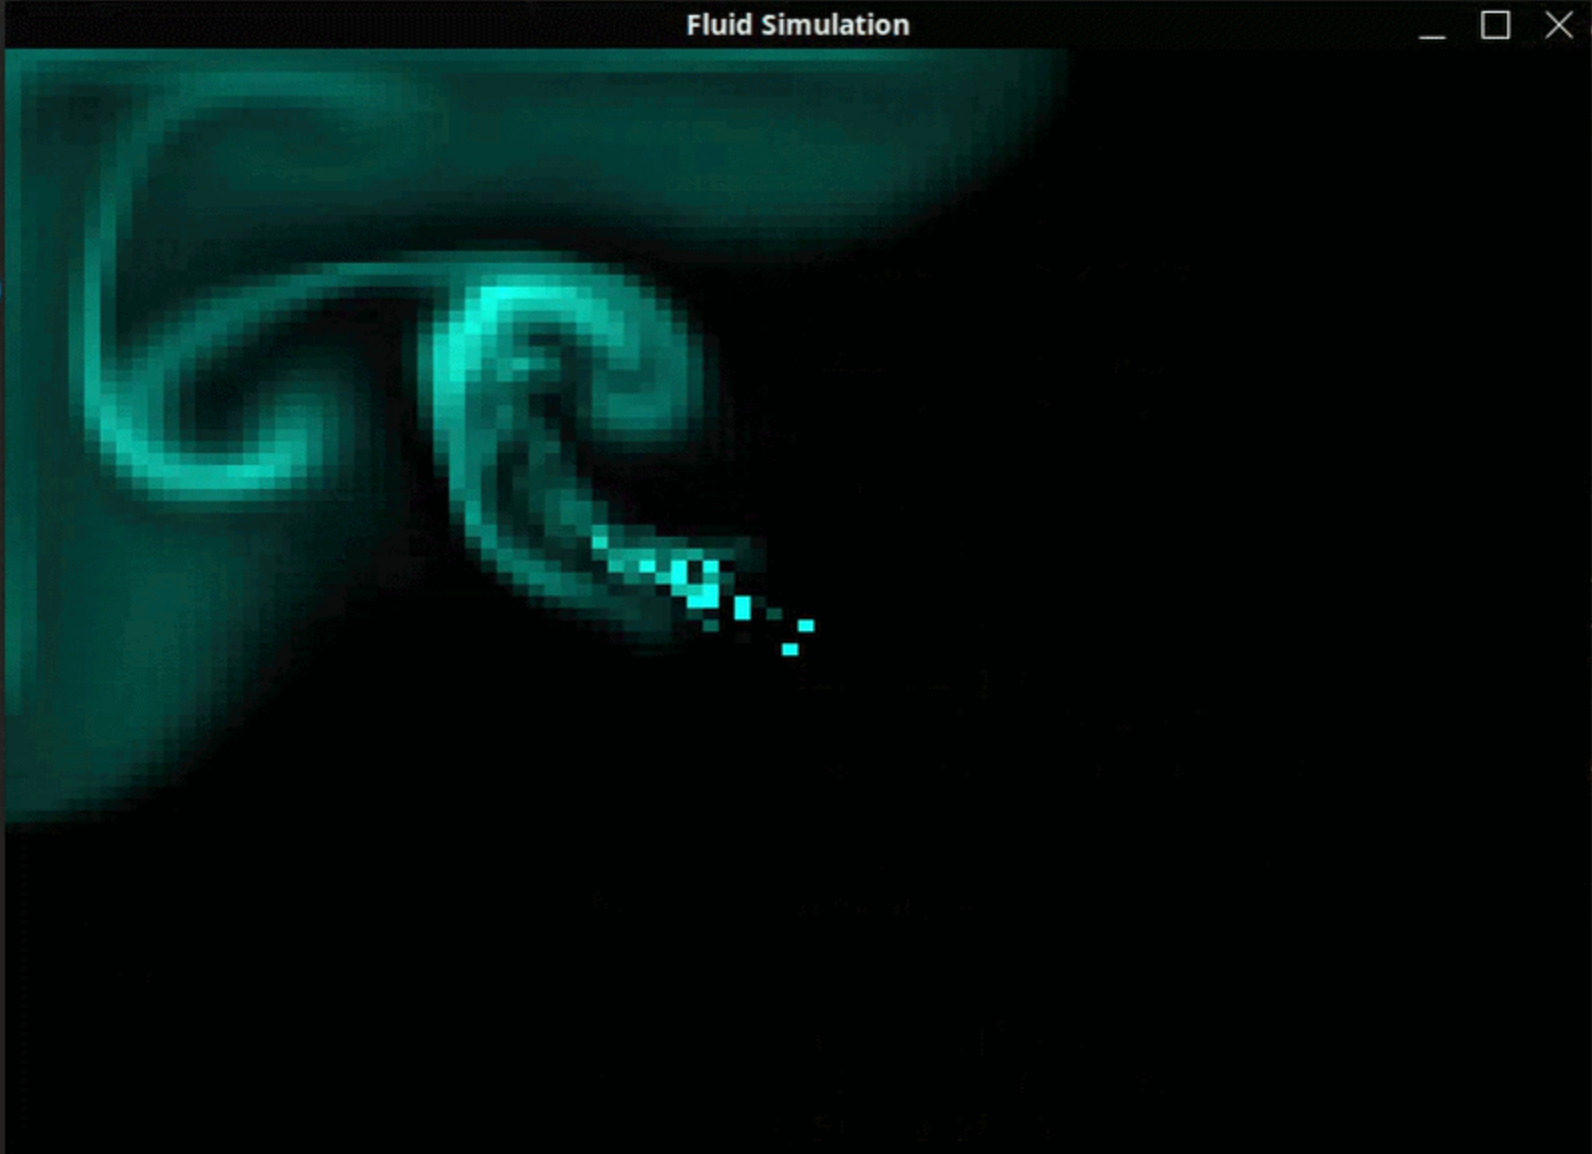
\includegraphics[width=0.45\textwidth]{../PJ_proj/simulation_evol1.png}
    \caption{Deuxieme version : affichage d'un fluide.}
    \label{figure2}
\end{figure}


\subsubsection{Panneau de paramètres (voir Figure~\ref{figure3})}
\comment{}{À déplacer dans la section "Interface Utilisateur" ?}
\gaelle {
    Notre affichage comporte un panneau de paramètres développé avec ImGui. Ce panneau nous permet de modifier en temps réel, lors de la simulation, différents paramètres tels que la densité, la couleur ou encore la direction du fluide. Les valeurs saisies par l'utilisateur sont envoyées au module de simulation qui met à jour la grille. Ce panneau peut être affiché ou masqué en pressant la touchant \texttt{h}.
}

\begin{figure}[H]
    \centering
    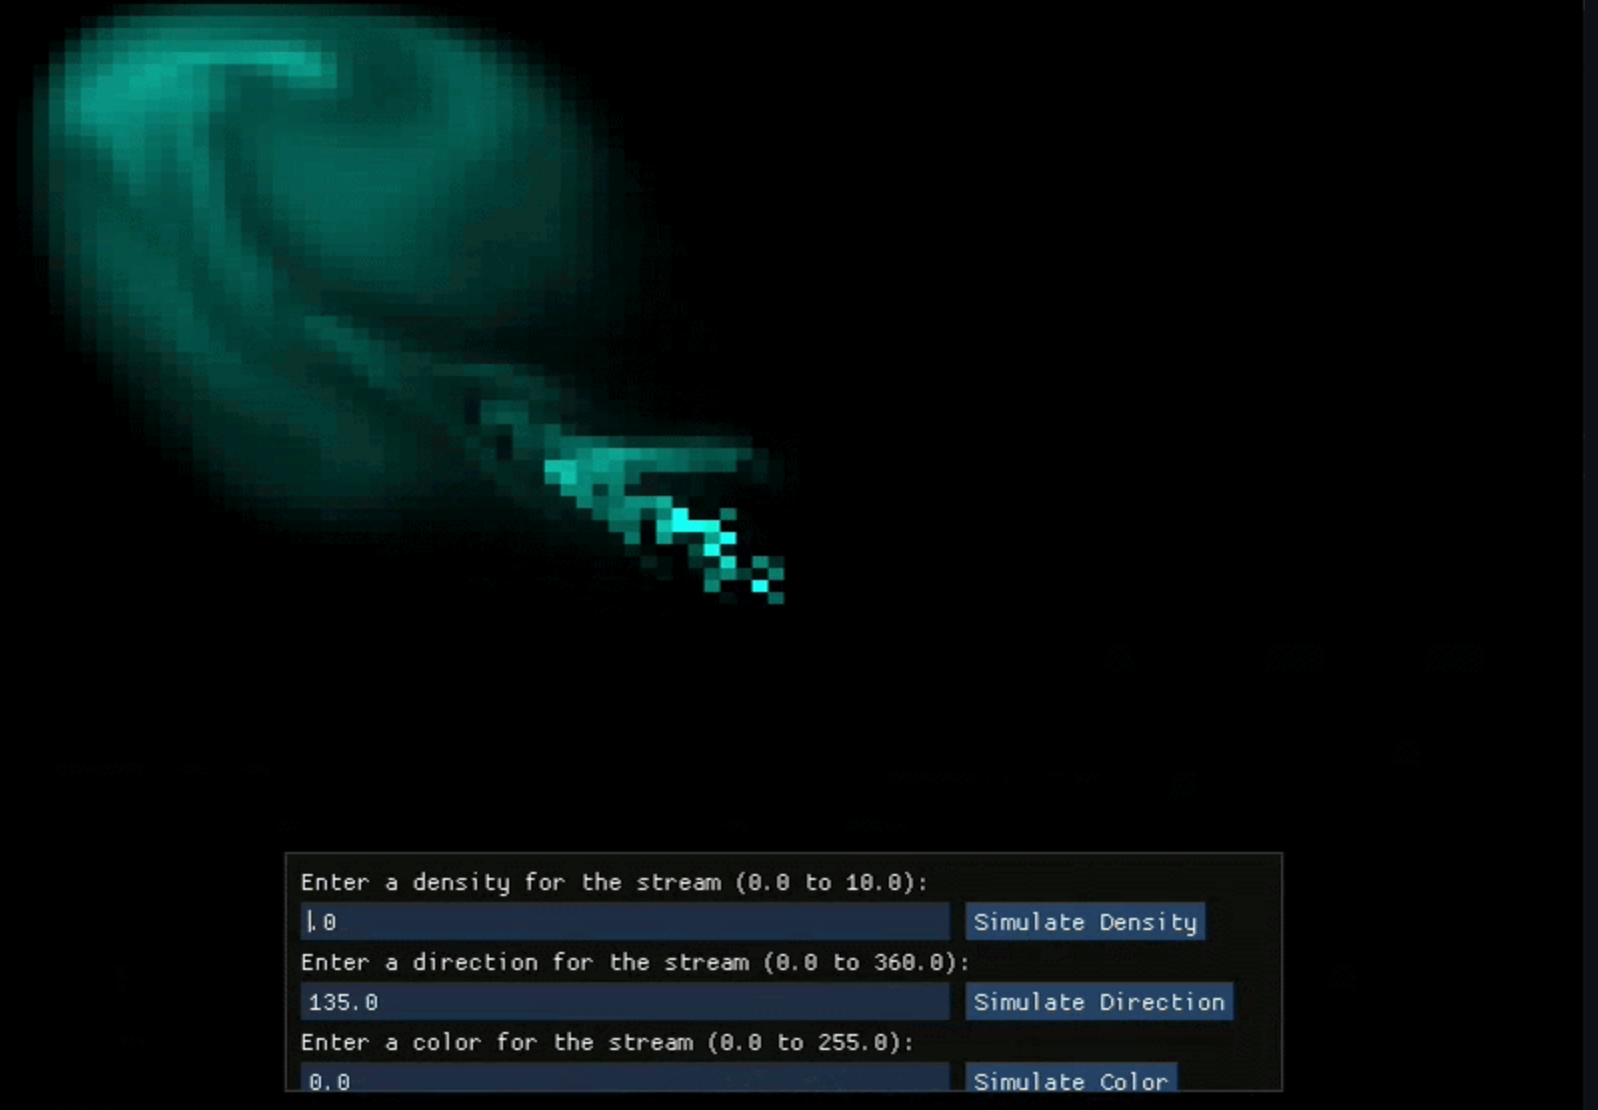
\includegraphics[width=0.45\textwidth]{../PJ_proj/simulation_evol2.png}
    \caption{Troisième version : ajout d'un panneau de paramètres.}
    \label{figure3}
\end{figure}


\subsubsection{Gestion des obstacles }
\gaelle {
L'affichage possède également un suystème de gestion des obstacles. L'utilisateur peut activer ou désactiver les obstacles, changer leur forme ou en ajouter plusieurs \add{Reference à la figure}. Chaque obstacle peut être déplacé grâce au curseur de la souris, cela nous permet d'observer son impact sur la simulation.
} 
\comment{}{Attention, gardez le même style. Ici, je conseille de retirer le gras du texte.}

\satine{
     Dans un premier temps, nous avons implémenté la création d'un \textbf{unique obstacle}, en modifiant notament la fonction de gestion des bords afin qu'elle reconnaise les obstacles. Nous pouvions également afficher ou non cet obstacle à l'aide d'un \textbf{bouton on/off} \add{Ajouter une image de ce bouton et ajouter une référence à la figure} qui nous rammener a  l'utlisation ou non de la fonction lancant la creation de l'obstacle.  Par la suite, nous avons rendu cet obstacle le plus \textbf{interactif} possible en offrant à l'utilisateur  la possibilité de le déplacer à l'aide du curseur de la souris.

    \comment{}{C'est quoi la fonction de gestion des bords ? Qu'est-ce que vous avez modifié dedans ? Au niveau programmation, ça demande quoi comme changements pour pouvoir déplacer un obstacle ? }

Nous avons ensuite enrichi notre simulation en ajoutant la possibilité de gérer  \textbf{plusieurs obstacles simultanément}, ainsi que de choisir leur forme parmi  un \textbf{cercle}, un \textbf{cœur} ou une \textbf{étoile}. Pour cela, nous avans implementer un curseur comptant le nombre d'obstacle par forme ainsi qu'un bouton +/- sur chaque forme possible afin de pouvoir  ajouter ou supprimer les differents obstacles. Les obstacles sont stockés dans une unique \textbf{liste} contenant leurs coordonnées (x, y), rayon et forme,  ce qui permet de les manipuler facilement (ajout, suppression, sélection et déplacement) tout en créant un ordre de priorité \add{Liste de priorité pour quoi ?}.  L'utilisateur peut ainsi ajuster dynamiquement le nombre d'obstacles via une interface dédiée.

Afin de représenter précisément les différentes formes et leurs interactions avec le fluide,  nous avons implémenté des fonctions mathématiques permettant, pour chaque point $(x,y)$,  de déterminer sa position par rapport à un obstacle (intérieur, extérieur ou bord).  Par exemple, dans le cas d'un cercle de centre $(cx,cy)$ et de rayon $r$, la distance au bord est donnée par : \[ d(x,y) = \sqrt{(x-cx)^2 + (y-cy)^2} - r \] Ainsi, si $d < 0$, le point est à l'intérieur \replace{de la boule}{du disque} (donc le fluide ne peut pas y pénétrer), si $d = 0$, il est sur le bord (donc le fluide est en contact avec l'obstacle), et si $d > 0$, il est à l'extérieur (donc le fluide peut y pénétrer). 

Pour des formes plus complexes comme le cœur, nous utilisons une \replace{représentation}{forme paramétrique} définie à l'aide d'un paramètre  $t \in [0, 2\pi]$ : \[ x(t) = 16 \sin^3(t) \] \[ y(t) = 13\cos(t) - 5\cos(2t) - 2\cos(3t) - \cos(4t) \] \cite{heartCurve}. Ces coordonnées sont ensuite normalisées, redimensionnées et translatées afin de positionner  correctement le cœur dans la simulation. Cette approche permet d'obtenir une forme realiste et cohérente.

\comment{De même, le triangle est conçu à partir de deux triangles equilatéraux.}{???}

Enfin, pour améliorer le plus possible le réalisme de la simulation, nous avons mis en place une gestion  des interactions entre le fluide et les obstacles. En utilisant en particulier, la fonction \texttt{obstacleNormal} qui  permet de calculer la \textbf{normale} au bord de chaque obstacle, c'est-à-dire la direction  perpendiculaire à sa surface. Cette information est essentielle pour simuler correctement  les phénomènes de réflexion et de rebond du fluide. Ainsi, le fluide réagit  de manière cohérente à la forme des obstacles, rendant la simulation realiste et représentatif. 

\comment{}{La normale sert à quoi ? Quand est-ce que vous l'utilisez ? Qu'est ce qui est réfléchit dans la simulation ? Qu'est-ce qui se passerait si vous ne réflechissiez pas les choses ?}

\replace{Voici ci-dessous une illustration de}{La figure \ref{evolution4b} illustre} l'ajout de plusieurs obstacles dans la simulation  (ici deux cercles, deux cœurs et une étoile à 6 branches) :
}


\begin{figure}[H]
    \centering
    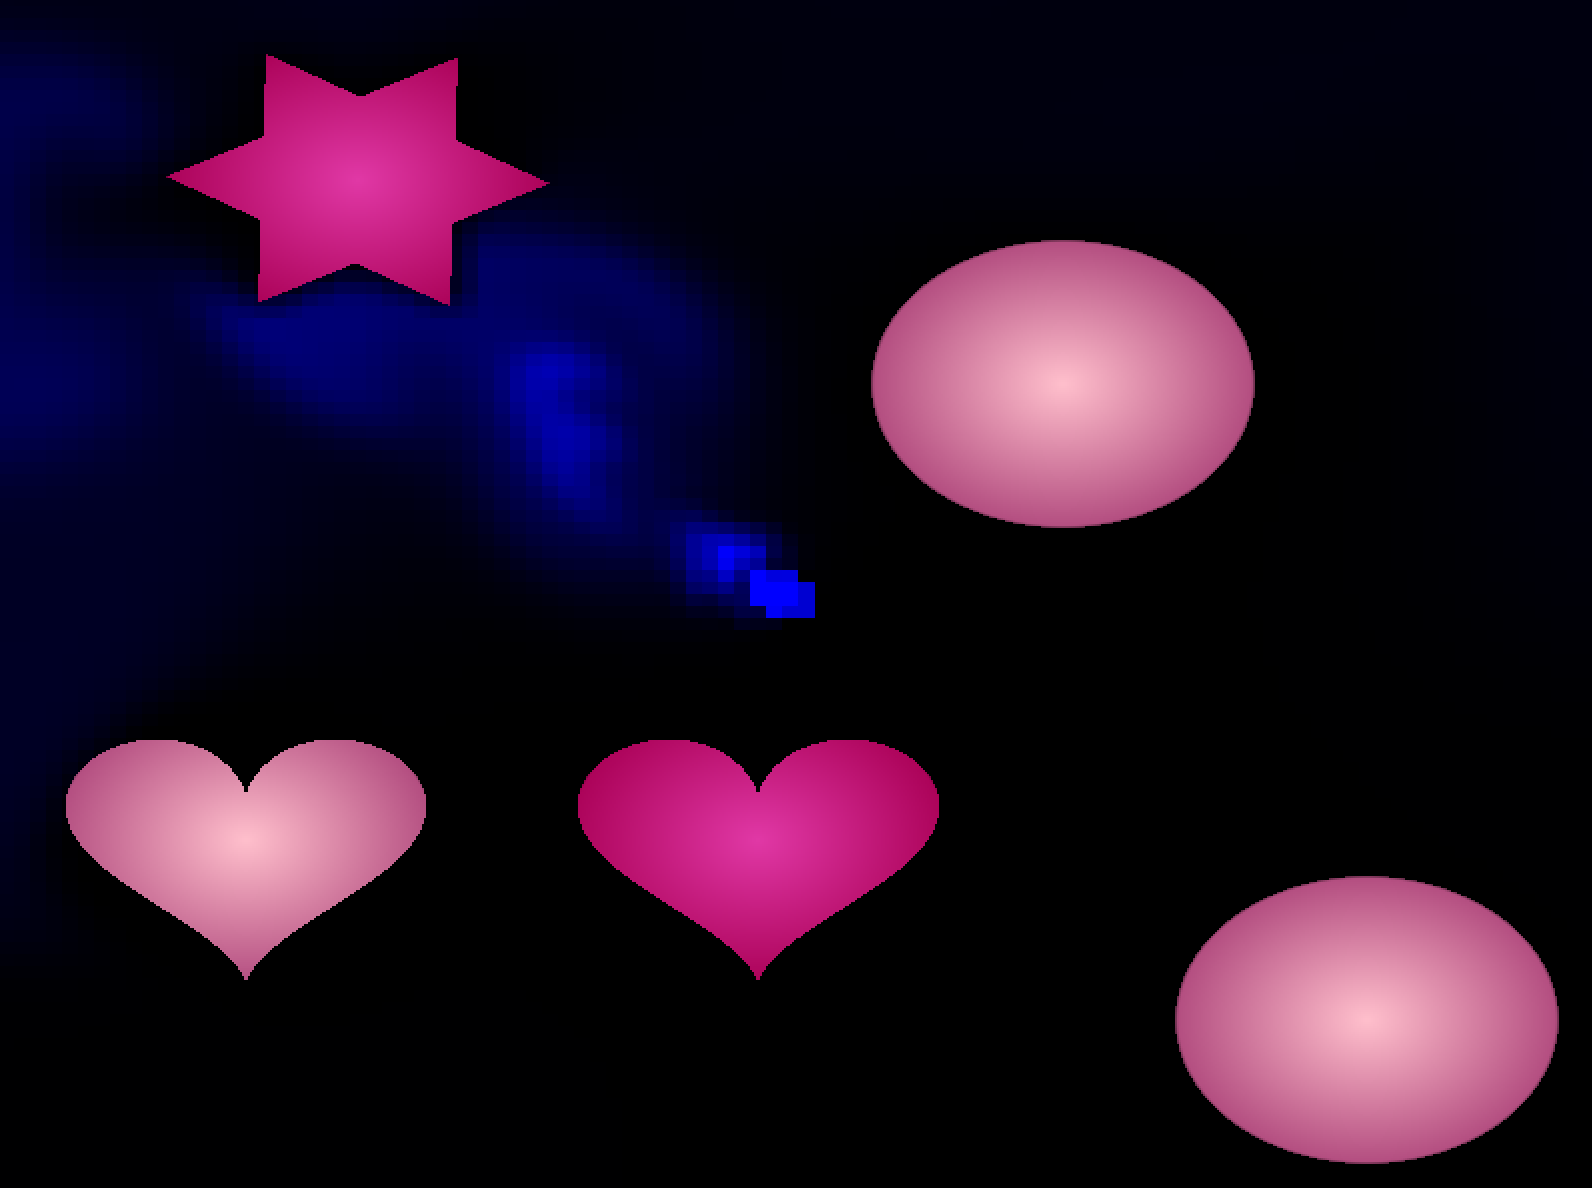
\includegraphics[width=0.45\textwidth]{../PJ_proj/tout_les_obstacles.png}
    \caption{Ajout de plusieurs obstacles.}
    \label{evolution4b}
\end{figure}


\subsubsection{Mode point/ligne}
\comment{}{Section "Interface Utilisateur" ?}
\gaelle {
    \replace{Dans l'interface il y a un paramètre permettant de choisir la forme de la source de fluide}{Le choix est donné à l'utilisateur de la forme de la source du fluide}. L'utilisateur peut injecter le fluide \add{provenant} soit en un point unique, soit le long d'une ligne définie par deux coordonnées dans la grille \remove{(soit 4 points)}.

    \comment{}{4 scalaires, non ? Ajouter un screenshot pour être plus clair.}

En mode point, la densité et les forces sont appliquées uniquement à la cellule correspondant à la position sélectionnée.

En mode ligne : nous déterminons simplement le nombre d'étapes nécessaires pour relier les deux points $(i_0,j_0),(i_1,j_1)$ en utilisant que le nombre d'étapes nécessaire est : 

$step = max(|i_1 - i_0|,|j_1 - j_0|)$. Lors ces étapes, nous parcourons, simplement toutes les cellules situées entre les deux positions sélectionnées, en suivant le segment qui les relie. Chaque cellule rencontrée reçoit la densité et la force, ce qui permet de créer une source linéaire.

}

\subsubsection{Gestion de la chaleur}
\comment{}{Section "Simulation" ?}
\sauranne {
Un mode d'affichage thermique permet de visualiser le fluide en fonction de sa température. Pour implémenter la chaleur dans notre simulation, nous avons ajouté un paramètre "chaleur" à chaque cellule de la grille. Ce paramètre est représenté par une valeur numérique qui peut être positive (indiquant une source chaude) ou négative (indiquant une source froide). 

Dans l'interface graphique, nous avons ajouté un bouton "Chaud/Froid" qui permet à l'utilisateur de choisir si le fluide injecté est chaud ou froid.

\begin{figure}[H]
    \centering
    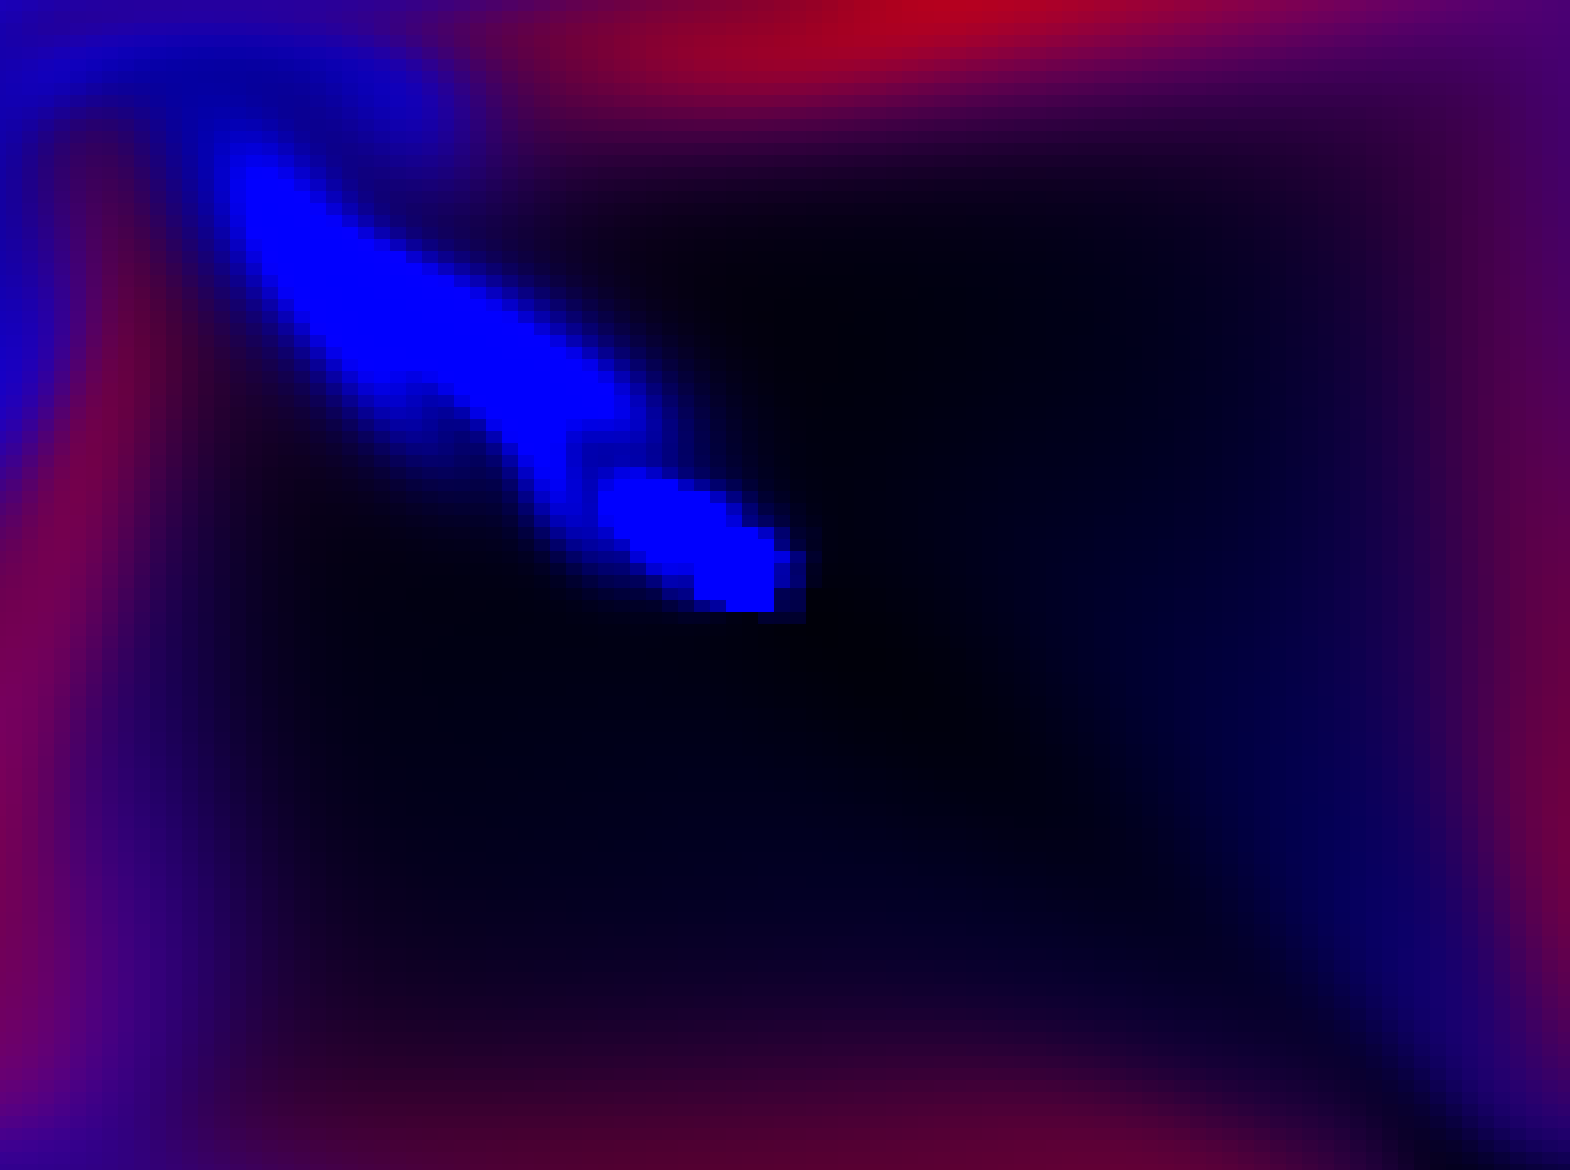
\includegraphics[width=0.45\textwidth]{../PJ_proj/bicolor.png}
    \caption{Affichage chaud/froid}
    \label{chaleur1}
\end{figure}

\replace{Sur cette image}{Dans la figure \ref{chaleur1}}, on peut voir l'état de la simulation après avoir alterné entre une source chaude (rouge) et une source froide (bleue). On observe quelques zones où les couleurs se mélangent (degradés de violet) ce qui correspond à des zones plutôt tièdes, mais aussi des zones où les couleurs sont très marquées et ne se mélangent pas. 


\begin{figure}[H]
    \centering
    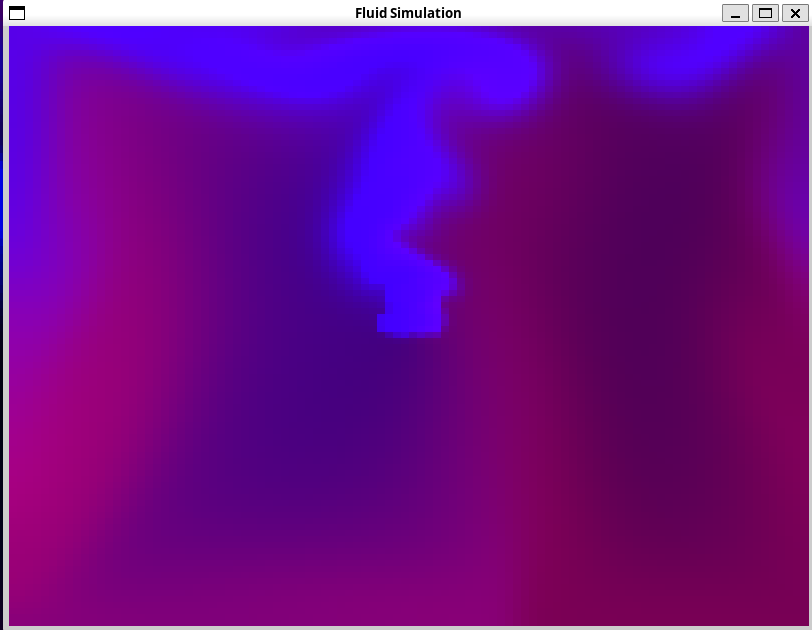
\includegraphics[width=0.45\textwidth]{../PJ_proj/chaleur.png}
    \caption{représentation température}
    \label{chaleur2}
\end{figure}

\replace{Ici}{Dans la figure \ref{chaleur2}}, on observe la simulation après de nombreuses itérations et on peut voir que le mélange est beaucoup plus homogène. On obtientcomme un voile violet, symbolisant une température tiède assez uniforme, avec quelques zones plus chaudes (rouge) ou plus froides (bleu). 

Ce mode d'affichage thermique peut être combiné avec les obstacles : 

\begin{figure}[H]
    \centering
    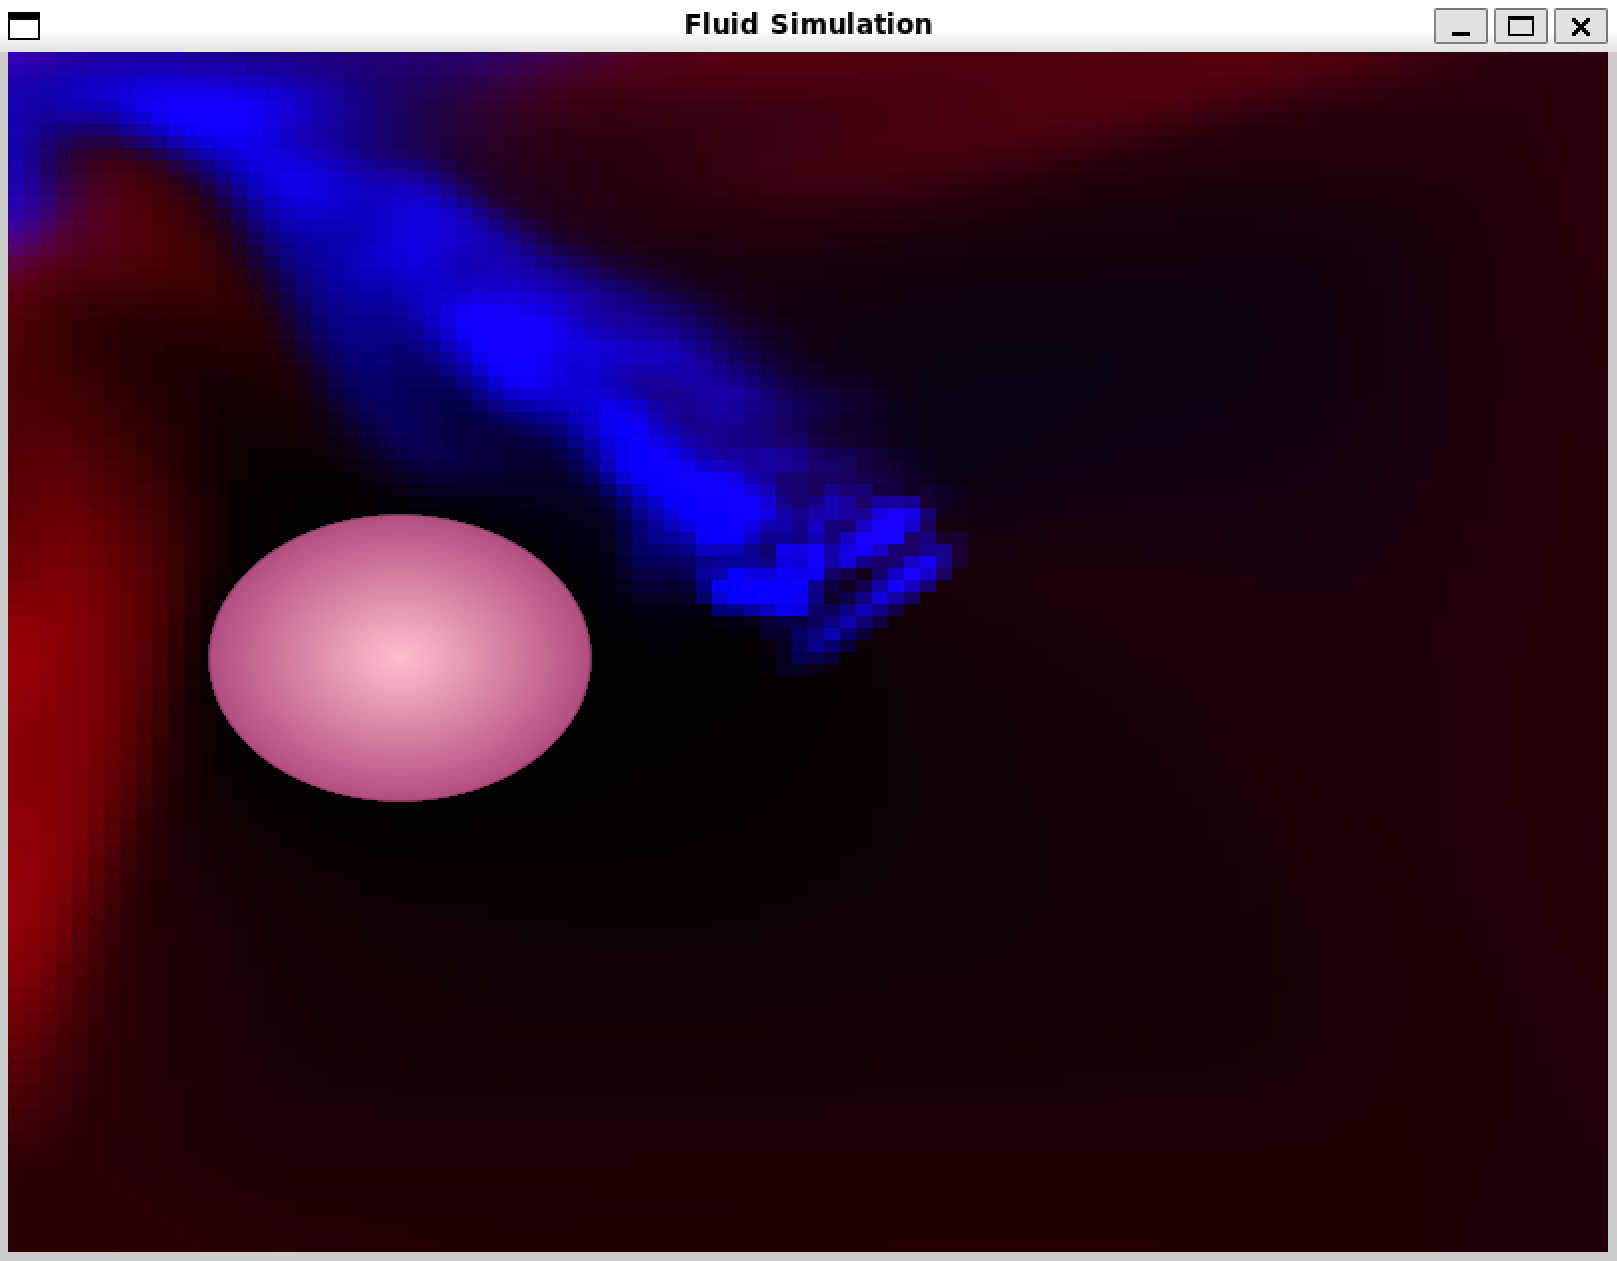
\includegraphics[width=0.45\textwidth]{../PJ_proj/simulation_evol3.png}
    \caption{chaleur + obstacles}
    \label{evolution4}
\end{figure}

On peut déplacer le cercle pour mélanger les différentes zones de temparature. Dans cette simulation, on considère que les obstacles sont neutres en terme de température, c'est à dire qu'ils n'ont pas d'effet de sur l'aspect thermique du fluide. 
}

% %2.3    SAURANE  -  GAËLLE  -  SATINE  -  AXEL
%   \item LES PARTIES SUIVANTES SONT A DEPLACER AU DESSUS
% \begin{itemize}
% %PARTIE A
% \label{2.3 - Partie A}
%   \item calcul d'une simulation, le fluide, physique
% %PARTIE B
%   \item PARTIE B :

% \label{2.3 - Partie B}
% \end{itemize}
\axel{
    \replace{Bluetooth, Semi-Lagrangien, Multi-threading}
    {\subsubsection{Modules en cours de développement}}
}

% ============================== AXEL 3 =======================================
\axel{
Nous avons envisagé plusieurs fonctionnalités dans notre projet que nous n'avons pas pu finaliser par manque de temps. 
\comment{}{Petit listing des 3 sous-modules}

\paragraph{Interface utilisateur sur smartphone}
Parmi elles, nous avons une interactivité avec la simulation non pas avec IMGUI depuis la fenêtre OpenGL mais avec une application depuis une machine externe. Une application de test et une gestion de port à des fins de transmissions de données ont été développées. Malheureusement sans qu'une connexion ne puisse être établie, et ceux depuis plusieurs téléphones avec l'application d'OS différentes couplés avec plusieurs ordinateurs sous Linux et Windows.
\comment{}{Divise tes phrases, elles sont trop longues.}

\paragraph{Semi-Lagrangien}
Pour enrichir notre simulation, nous souhaitions implementer une méthode semi-lagrangienne. Le semi-Lagrangien étant une méthode de simulation hybride entre l'Eulérien (utilisation de grilles à paramètres) et du Lagrangien (utilisation de particules au comportement régi par des lois \add{physiques}) nous voulions utiliser notre grille déjà existante (mentionnée dans la partie \underline{\emph{\nameref{2.3 - Partie A}}}\add{Voir dans un commentaire au-dessus comment se référer à une autre section}) afin d'y capturer notre simulation Lagrangienne de quelques particules. Une revisite de notre structure fût effective, nous avons redéfini notre structure-Singleton (référence, accessible de partout) en Structure Simulation : qui contient une structure grille, et notre nouvelle structure particules qui est \replace{grossièrement}{principalement} un vecteur de structure particule, relativement analogue à la structure Cell (cellules de la grille). \add{Référence à l'UML, ou ajout d'une figure avant/après de votre UML.}

\paragraph{Calcul parallèle}
Une approche de parallélisme a été envisagée ; nous avons installé OpenMP pour faire donc du \emph{Multi-Processing} sur OpenGL afin de pouvoir se permettre d'augmenter la résolution (taille de grille) de notre simulation, mais nous n'avons pu faire aboutir cette option par faute de temps.
}

%2.4      AXEL
\subsection{Interface utilisateur}
\label{sec:interface-utilisateur}
% ============================== AXEL 4 =======================================
\axel{
    Notre panneau d'interaction avec la simulation permet de mettre la main sur \replace{un panel de parties arbitraires}{de nombreuses variables} de notre simulation. Nous avons essayé de faire en sorte que chaque variable arbitraire devienne un curseur, une valeur à saisir, un interrupteur à enclencher afin de rendre notre simulation riche en personnalisation \add{Ajouter une image avec ces différents inputs}. De ce fait, nous pouvons (entre autres) modifier la densité du fluide, sa force, sa direction, la disposition du/des points de départs sa couleur aussi. Nous avons aussi des obstacles que nous pouvons ajouter, on peut choisir leur nombre, leurs formes ainsi que leur position avec un simple clic avec déplacement de la souris.
}
\begin{itemize}
    \item description des boutons et des interactions possibles
\end{itemize}
%2.5       AXEL
\subsection{Format des données d'entrée}
\begin{itemize}
    \item fluide stocké dans une grille
    \item grille composée de cellules
    \item cellules contiennent les paramètres de la simulation (densité, chaleur, vitesse)
    \item expliquer ce que représentent ces paramètres

% ============================== AXEL 5 =======================================
\axel{
Notre encodage des données se fait majoritairement via des \replace{flottants}{scalaires}. Le fluide se décompose en plusieurs données physiques (densité, pression, viscosité, \emph{etc...}) que l'on encode via des flottants et que l'on stock dans une structure Cell (cellule) dont on forme un vecteur d'ensemble dans une structure Grid (grille). Dans ce genre de structure on implémente des attributs-méthodes de tailles en \replace{integers}{entiers}. On perfectionne notre diversité de simulation avec des conditions booléenne pour savoir si oui ou non, on affiche un obstacle, si oui ou non on a plusieurs points de fuites, \emph{etc ...}

}
%2.6     SAURANE
\end{itemize}

\subsection{Statistiques}
\sauranne {
    En termes de statistiques, notre projet est composé de certaines classes principales : Cellule, Grille, Obstacle, etc. Il est composé de 22 fichiers (cpp et h), et contient plus de 2000 lignes de code. Le projet est organisé en plusieurs modules, tels que le module de gestion des obstacles, le module de gestion de la chaleur, etc.

    \comment{}{Ajouter un tableau avec les fichiers pour chaque module, et pour chaque fichier, son nombre de lignes.}
}
% \end{enumerate}

\section{Algorithmes et Structures de Données}
\remove{\emph{2 à 3 pages}}
% \begin{enumerate}%pour faire une liste numérotée
%3.1        GAËLLE  -  SATINE  -  SAURANE
\subsection{Principaux algorithmes utilisés}

\sauranne {
     Dans cette section, nous allons présenter et analyser l'un des algorithmes principaux du projet : \texttt{vel\_step}. Pour cela, nous allons détailler 3 algorithmes essentiels : advection, diffusion et projection. \texttt{vel\_step} est l'algorithme qui fait évoluer la vitesse du fluide à chaque itération de la simulation.
}
\begin{verbatim}
    Algorithme : vel_step
        Début
            ajouter_source(N, u, u_prev, dt)
            ajouter_source(N, v, v_prev, dt)

            Echanger u et u_prev

            diffuse(N, 1, u, u_prev, visc, dt)
            Echanger v et v_prev
            diffuse(N, 2, v, v_prev, visc, dt)

            project(N, u, v, u_prev, v_prev)

            Echanger u et u_prev, Echanger v et v_prev
            advect(N, 1, u, u_prev, u_prev, v_prev, dt)
            advect(N, 2, v, v_prev, u_prev, v_prev, dt)

            project(N, u, v, u_prev, v_prev)
        Fin
\end{verbatim}

\comment{}{On a besoin de savoir ce que ça fait, tout ça ! C'est quoi "N", "u", "v\_prev", "dt", etc...! Structure de données (scalaire, tableau de scalaire ?) et description ("vélocité précédente verticale/horizontale", "pas de temps" ?)}


\subsubsection{Advection}
\gaelle {
L'advection est un processus physique qui décrit le transport d'une quantité (densité, chaleur ou vitesse) par le fluide.L'advection déplace l'information en suivant le mouvement du fluide. Dans \replace{notre simulation}{le travail de Jos Stam \cite{Stam99}}, nous utilisons l'approche \emph{semi-lagrangienne} introduite. L'équation de l'advection est  :
\[
    \frac{\partial x}{\partial t} + \mathbf{u} \cdot \nabla x = 0,
\]
où $x$ est la quantité transportée et $\mathbf{u} = (u,v)$ le champ de vitesse. L'idée est de déterminer, pour chaque cellule $(i,j)$, la position d'où provient le fluide arrivé à cet endroit au temps $t + \Delta t$. On remonte donc le long du champ de vitesse :
\[
    x' = i - \Delta t \cdot N \cdot u(i,j), \qquad y' = j - \Delta t \cdot N \cdot v(i,j).
\]
\comment{}{C'est quoi "N" ? Le nombre de lignes/colonnes. Pourquoi il est inclut ici ? Si c'est pas facile à expliquer, donc je conseille de le retirer des formules. (elles restent correctes, promis)}

Comme $(x',y')$ n'est généralement pas un point entier de la grille, on utilise une \emph{interpolation bilinéaire} entre les quatre cellules voisines pour estimer la valeur transportée.
}

\remove{\paragraph{Pseudo-code de l'advection}}
\begin{verbatim}
    fonction ADVECT(N, b, d, d0, u, v, dt)

        dt0 ← dt × N

        pour i de 1 à N faire
            pour j de 1 à N faire
                
                # 1. Remonter le long du champ de vitesse
                x ← i - dt0 × u[i,j]
                y ← j - dt0 × v[i,j]

                # 2. Contraindre la position dans la grille
                si x < 0.5 alors x ← 0.5
                si x > N + 0.5 alors x ← N + 0.5
                si y < 0.5 alors y ← 0.5
                si y > N + 0.5 alors y ← N + 0.5

                i0 ← floor(x)
                i1 ← i0 + 1
                j0 ← floor(y)
                j1 ← j0 + 1

                # 3. Coefficients d'interpolation
                s1 ← x - i0
                s0 ← 1 - s1
                t1 ← y - j0
                t0 ← 1 - t1

                # 4. Interpolation bilinéaire
                d[i,j] ← 
                    s0 × ( t0 × d0[i0,j0] + t1 × d0[i0,j1] ) + 
                    s1 × ( t0 × d0[i1,j0] + t1 × d0[i1,j1] )

            fin pour
        fin pour

        appliquer_conditions_aux_limites(d)

    fin fonction
\end{verbatim}

\comment{}{Pareil, décris les entrées et ce qu'elles représentent.}

\gaelle{
L'advection semi-lagrangienne peut être vue comme un déplacement de matière : au lieu de pousser la matière vers l'avant, on cherche d'où elle provient et on la pousse dans la direction continue. Visuellement, l'advection est responsable du mouvement du fluide.
}

\subsubsection{Diffusion}
\satine{
Comme l'advection, la diffusion est un processus physique qui décrit la propagation d'une substance. Nous avons donc choisit de l'implementer en pseudocode comme suit :
}

\begin{verbatim}
    fonction DIFFUSE(N, x, x0, diff, dt)
        a ← dt × diff × N²

        pour k de 1 à 20 faire
            pour i de 1 à N faire 
                pour j de 1 à N faire     
                    x[i,j] ← ( x0[i,j]             
                            + a × ( x[i-1,j] + x[i+1,j]     
                            + x[i,j-1] + x[i,j+1] ) )             
                            / (1 + 4a) 
                fin pour
            fin pour

            appliquer_conditions_aux_limites(x)
        fin pour

        retourner x

    fin
\end{verbatim}

\satine{
L'algorithme de diffusion utilise l'equation aux derivées partielles qui suivent :
\begin{equation*}
    \frac{\partial x}{\partial t} = D \nabla^2 x
\end{equation*}

où :
\begin{itemize}
    \item $x$ est la quantité diffusée (densité, température),
    \item $D$ est le coefficient de diffusion,
    \item $\nabla^2$ est le Laplacien.
\end{itemize}

En utilisant la discretisation utiliser par Jos Stam on obtient :
\begin{equation*}
    x^{t+1} = x^t + \Delta t \, D \, \nabla^2 x^{t+1}
\end{equation*}

Ce choix est essentiel pour garantir la stabilité numérique, même pour de grands pas de temps. Sur une grille 2D, le Laplacien discret est approximé par :
\begin{equation*}
    \nabla^2 x_{i,j} \approx x_{i-1,j} + x_{i+1,j} + x_{i,j-1} + x_{i,j+1} - 4x_{i,j}
\end{equation*}

En remplacant la formule de Jos Stam par l'approximation du Laplacien, on obtient :
\begin{equation*}
    x_{i,j}^{t+1} = \frac{x_{i,j}^{0} + a \left(x_{i-1,j}^{t} + x_{i+1,j}^{t} + x_{i,j-1}^{t} + x_{i,j+1}^{t}\right)}{1 + 4a}
\end{equation*}

avec :
\begin{equation*}
    a = \Delta t \cdot D \cdot N^2
\end{equation*}

D'après Gauss-Seidel, l'équation précédente correspond à un système linéaire de la forme :
\begin{equation*}
    (I - a \Delta)x = x_0
\end{equation*}

Ce système est résolu par une méthode itérative de Gauss-Seidel. Elle consiste à :
\begin{itemize}
    \item parcourir la grille plusieurs fois,
    \item mettre à jour chaque cellule immédiatement avec les nouvelles valeurs disponibles,
    \item répéter jusqu'à convergence.
\end{itemize}

Cette méthode accélère la convergence et permet une simulation stable et efficace. Ainsi, on peut interpréter la diffusion comme un processus qui rend les valeurs de plus en plus uniformes : Une zone où la quantité est très concentrée se diffuse progressivement vers les cellules voisines. Au fil des itérations, cela rend la répartition de plus en plus uniforme, ce qui est indispensable pour obtenir des simulations de fluides réalistes.
}

\subsubsection{Projection}
\sauranne {
    Après avoir appliqué les algorithmes d'advection et de diffusion, l'algorithme de projection implémente \comment{la décomposition de Hodge.}{Si vous le laissez, sachez que ça tombera sûrement en tant que question du jury à la soutenance, ça.} 
    C'est un algorithme qui permet de rendre le champ de vitesse du fluide incompressible et qui force la vitesse à conserver la masse. C'est une propriété importante des fluides réels. 

Visuellement, la projection force l'écoulement à avoir de meilleures courbes, et évite les écoulements en ligne droite. 

La décomposition de Hodge nous dit que tout champ de vecteur de vitesse est la somme d'un champ conservant la masse et d'un champ de gradient. L'idée est de rendre le champ de vitesse conservateur de masse lors de la dernière étape en soustrayant le champ de gradient du champ de vitesse actuel.
}

\begin{verbatim}
    Algorithme : Projection
        Entrées : int N, float * u, float * v, float * div, float * p
        Sorties : u et v modifiés pour être incompressibles

        Début
            h = 1.0 / N

            # ÉTAPE 1
            Pour chaque cellule (i, j) de la grille :
                div[i, j] = -0.5 * h * (u[i+1, j] - u[i-1, j] + v[i, j+1] - v[i, j-1])
                p[i, j] = 0
            Fin Pour
            Appliquer les bords pour 'div' et 'p'

            # ÉTAPE 2
            Répéter 20 fois :
                Pour chaque cellule (i, j) de la grille : 
                    p[i, j] = (div[i, j]  + p[i-1, j] 
                              + p[i+1, j] + p[i, j-1] 
                              + p[i, j+1]) / 4
                Fin Pour
                Appliquer les bords pour 'p'
            Fin Répéter

            # ÉTAPE 3 :
            Pour chaque cellule (i, j) de la grille :
                u[i, j] = u[i, j] - 0.5 * (p[i+1, j] - p[i-1, j]) / h
                v[i, j] = v[i, j] - 0.5 * (p[i, j+1] - p[i, j-1]) / h
            Fin Pour
            Appliquer les bords pour 'u' et 'v'
        Fin
\end{verbatim}
\comment{}{Veillez à avoir un style visuel identique entre les pseudo-codes.}

\sauranne{
L'algorithme de projection est composé de 3 étapes : 

% \begin{itemize}
    \paragraph{Etape 1 :} calcul de la divergence : pour chaque cellule de la grille, on évalue la divergence discrète
\begin{equation}
    {div}_{i,j} = -\frac{h}{2}(u_{i+1,j} - u_{i-1,j} + v_{i,j+1} - v_{i,j-1})
\end{equation}

où $h = 1/N$ est la taille d'une cellule de la grille, et $u$ et $v$ sont les composantes de la vitesse du fluide. 

    \paragraph{Etape 2 :} résolution de l'équation de Poisson 

On résout itérativement l'équation $\nabla^2 p = div$ par 20 itérations de relaxation de Gauss-Seidel, où $p$ est un champ de pression :
\begin{equation}
p_{i,j}^{(k+1)} = \frac{1}{4}({div}_{i,j} + p_{i+1,j}^{(k)} + p_{i-1,j}^{(k)} + p_{i,j+1}^{(k)} + p_{i,j-1}^{(k)} - div_{i,j})
\end{equation}

On réutilisa exactement le code de la diffusion pour assurer la cohérence du code et éviter les redondances. 

    \paragraph{Etape 3 :} correction du champ de vitesse 

pour chaque cellule de la grille, on corrige la vitesse en soustrayant le gradient du champ de pression :
\begin{align}
    u'_{i,j} &= {u}_{i,j} - \frac{1}{2h} ( p_{i+1,j} - p_{i-1,j})  \\
    v'_{i,j} &= {v}_{i,j} - \frac{1}{2h} ( p_{i,j+1} - p_{i,j-1})
\end{align}

% \end{itemize}
}

%3.2        GAËLLE  -  SATINE  -  SAURANE
\subsection{Complexité théorique en temps des algorithmes présentés}

\sauranne {
    Les algorithmes d'advection, de diffusion et de projection nous permettent de définir l'algorithme \texttt{vel\_step}. Sa complexité en temps est déterminée par les 3 algorithmes principaux qui la composent :

\paragraph{Advection.}
L'algorithme d'advection met à jour la valeur de la densité ou la vitesse pour chaque cellule de la grille. L'algorithme parcourt donc toute la grille de taille $N \times N$ avec une double boucle \emph{for}, ce qui représente $N^2$ cellules.

Pour chaque cellule, l'algorithme
\begin{itemize}
    \item détermine la position d'origine du fluide
    \item effectue une interpolation
    \item met à jour la valeur de la desnité ou vitesse
\end{itemize}
Toutes ces opérations sont réalisées en temps constant ($\mathcal{O}(1)$) pour chaque cellule. Alors avec la double boucle, on obtient un coût total de $N^2 \times \mathcal{O}(1) = \mathcal{O}(N^2)$.

A la fin de l'algorithme, il y a un appel à la fonction \emph{set\_bnd} qui a une complexité $\mathcal{O}(N^2)$.

La complexité finale de l'algorithme \emph{advection} est donc : 

$$\mathcal{O}(N^2) + \mathcal{O}(N^2) = \mathcal{O}(N^2)$$.

\paragraph{Diffusion.}
\satine{L'algorithme parcourt une grille de taille $N \times N$ à chaque itération, ce qui représente un coût de $N^2$.
Comme le nombre d'itérations est constant (20), la complexité totale est en $\mathcal{O}(N^2)$.
}

\paragraph{Projection.}
L'algorithme de projection est composé de 3 étapes :
\begin{itemize}     
    \item Etape 1 : calcul de la divergence : $N^2$ opérations  
    \item Etape 2 : résolution de l'équation de Poisson : $20 \times N^2$ opérations     
    \item Etape 3 : correction du champ de vitesse : $N^2$ opérations
\end{itemize}

Ainsi, la complexité totale de l'algorithme de projection est en $\mathcal{O}(N^2)$.

Ce qui nous donne une complexité totale de $\mathcal{O}(N^2 + N^2 + N^2) = \mathcal{O}(N^2)$ pour l'algorithme \texttt{vel\_step}.
}
\comment{}{Je recommande d'utiliser N=nombre de cellules plutôt que N=nombre de lignes. (donc juste diviser toutes les complexités par N)}
% \end{enumerate}


\section{Analyse des résultats }
\remove{\emph{2 à 4 pages}}
\remove{L'analyse expérimentale sera faites dans cette section. Elle sera plus ou moins importante dans votre projet comme pour les deux points précédent, cette section devra donc être développée en conséquence.}

% \begin{enumerate}%pour faire une liste numérotée
\remove{Illustrer les performances ainsi que l'efficacité du logiciel implémenté à l'aide de graphiques.}

\begin{itemize}
    \item calcul de complexités en fonction de la taille de la grille, etc (plot sur python), nombre d'obstacles, étape d'avection/relaxation (changer les paramètres et comparer)
\end{itemize}

\remove{Analyser (et comparer, si plusieurs) les performances des solutions implémentées.}
\begin{itemize}
    \item eulerien vs lagrangien (uniquement eulerien a été implémenté)
    \item analyser les performances visuelles en fonction du nombre d'obstacles, densité, etc (mettre des screenshot)
\end{itemize}

\satine{
    On peut voir l'évolution de notre projet a travers son evolution visuelle. mais egalement c'est peformance en fonction de différents paramètres tels que la densité du fluide ou le nombre d'obstacles.
}

\begin{figure}[H]
    \centering
    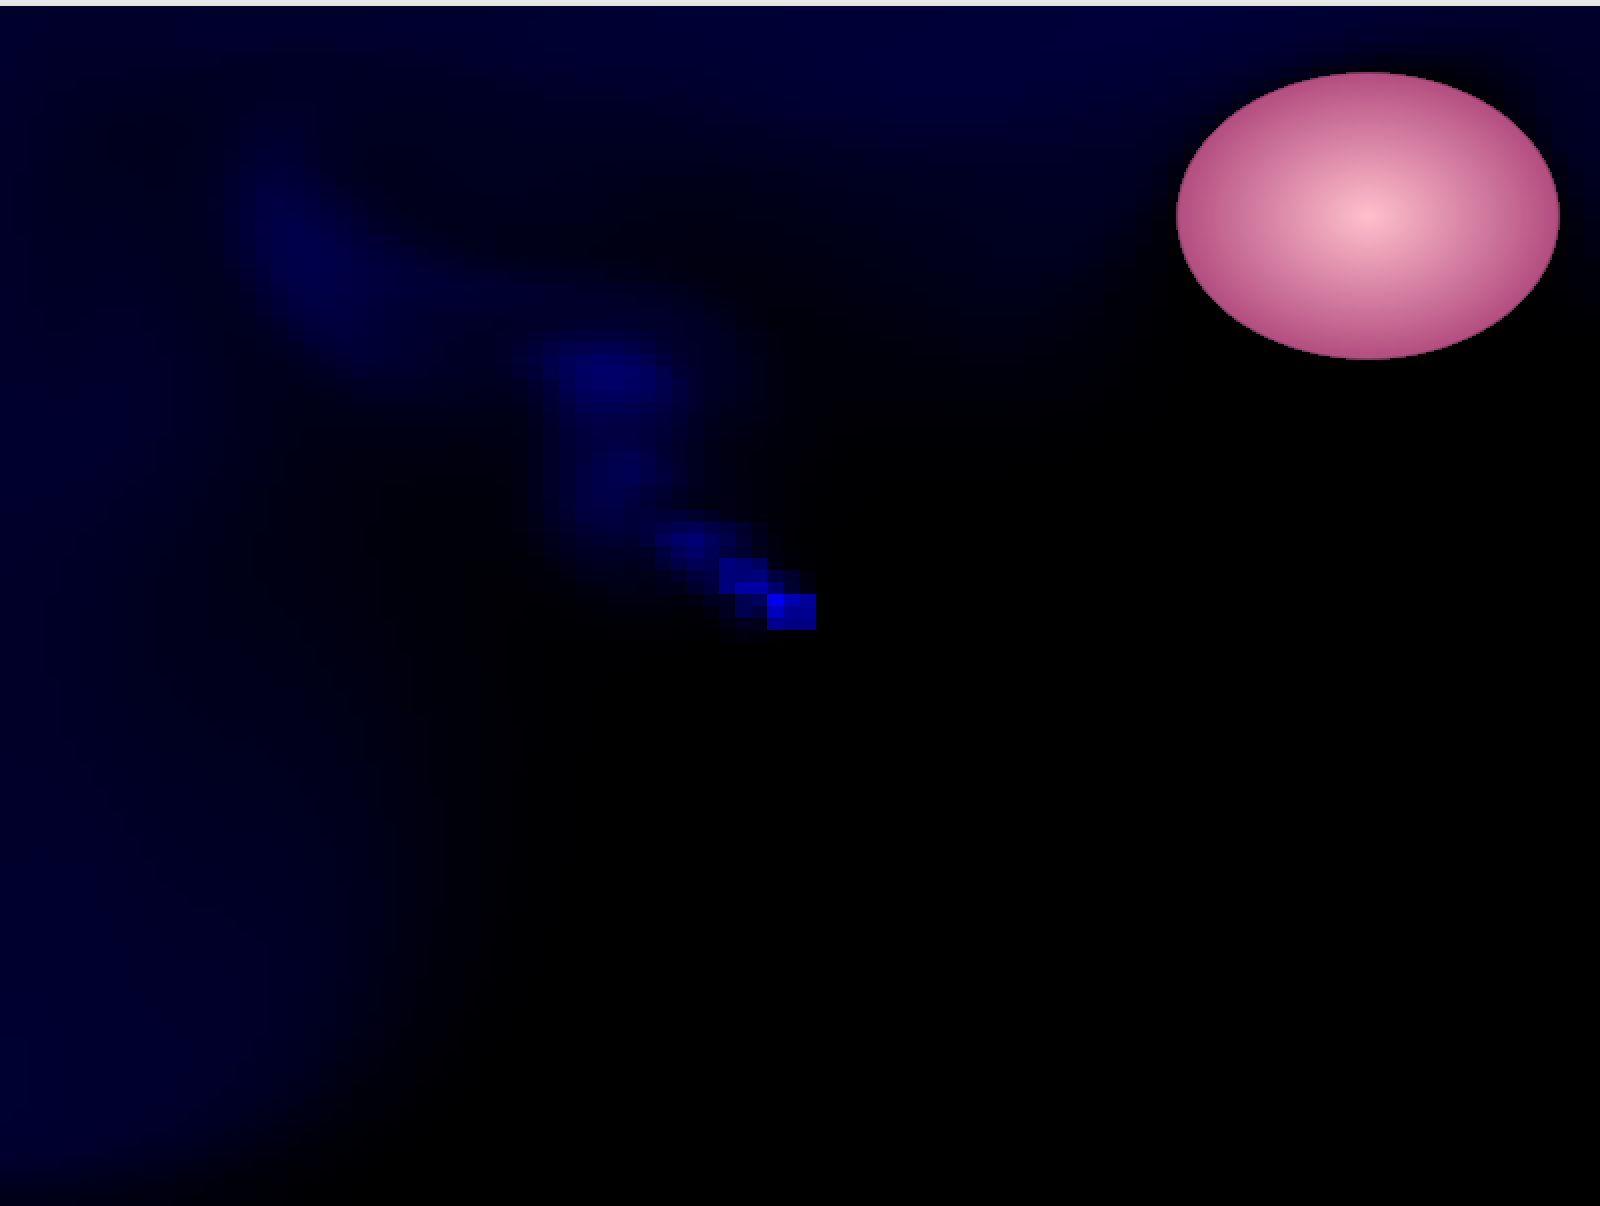
\includegraphics[width=0.45\textwidth]{../PJ_proj/image de base.png}
    \caption{Simulation avec un obstacle et toute les proprite du fluides non modifiées}
\end{figure}


\begin{figure}[H]
    \centering
    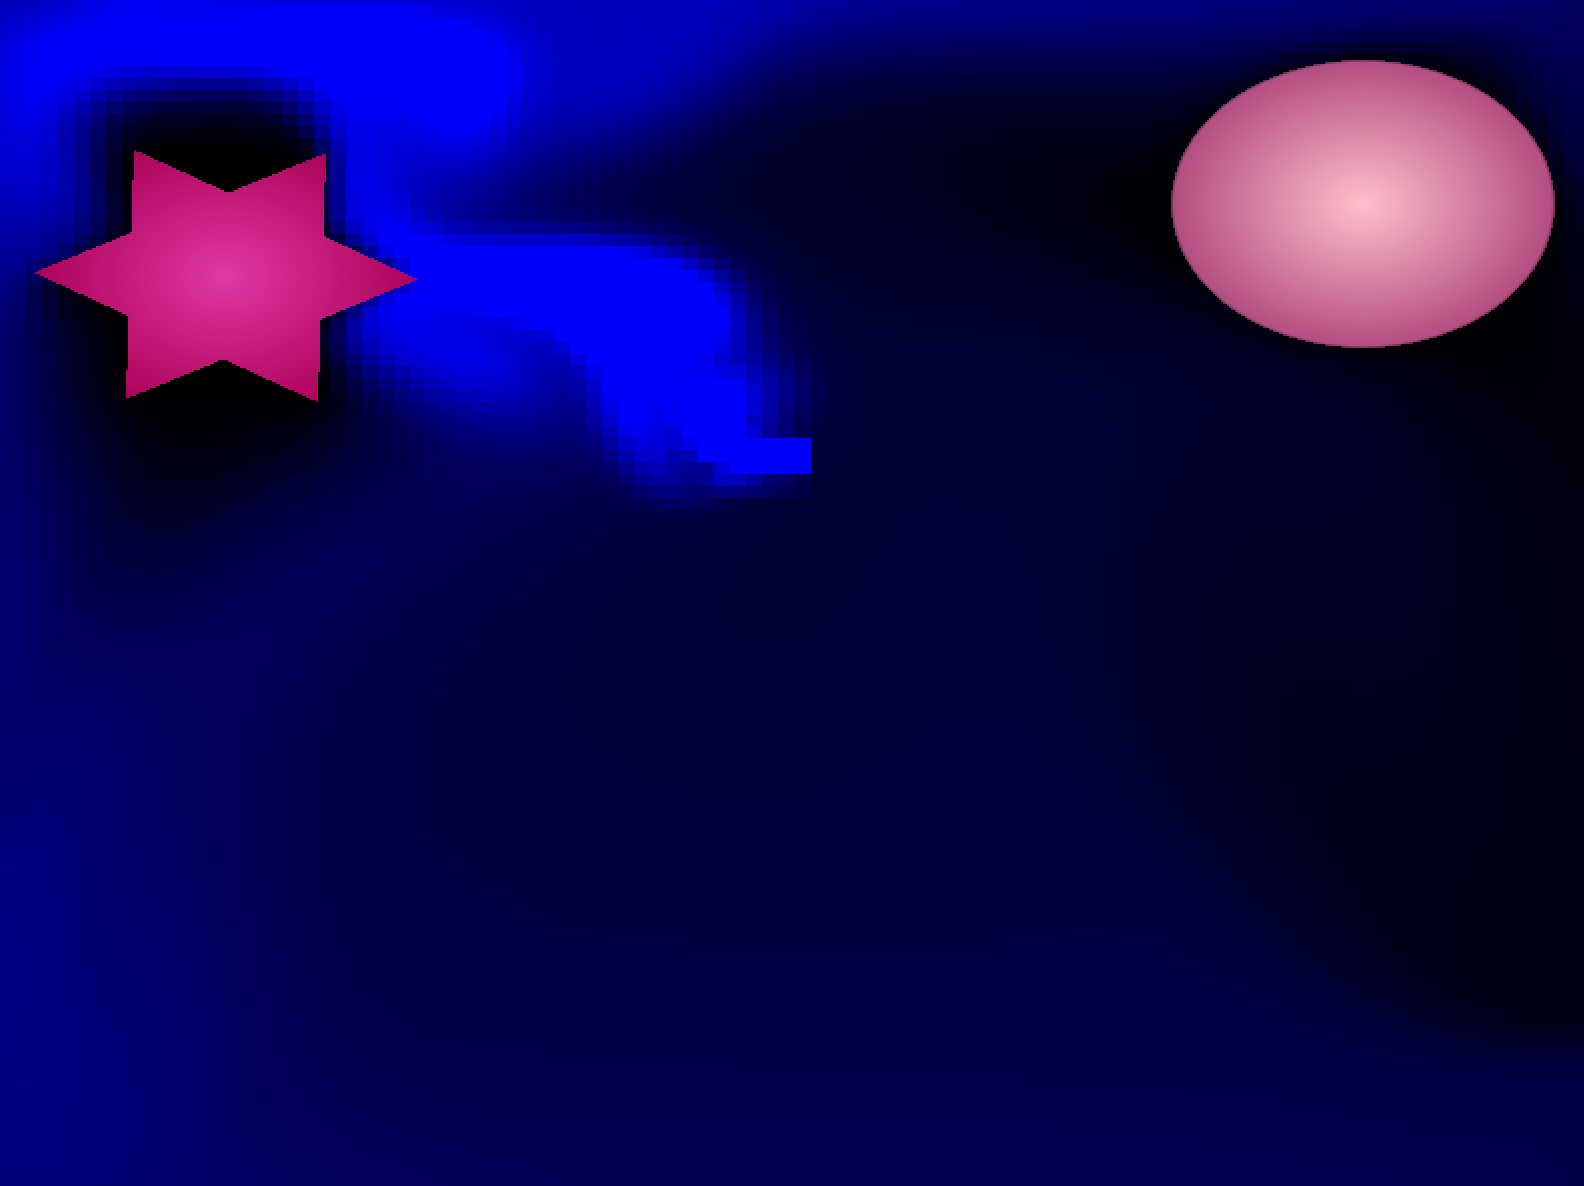
\includegraphics[width=0.45\textwidth]{../PJ_proj/densite 5_autre position.png}
    \caption{Simulation avec 2 obstacles et une densité plus élevée(5)}
\end{figure}

\satine{
    On constate une meillieur visibilite des obstacle et du fluide ainsi que sa direction.
}

\begin{figure}[H]
    \centering
    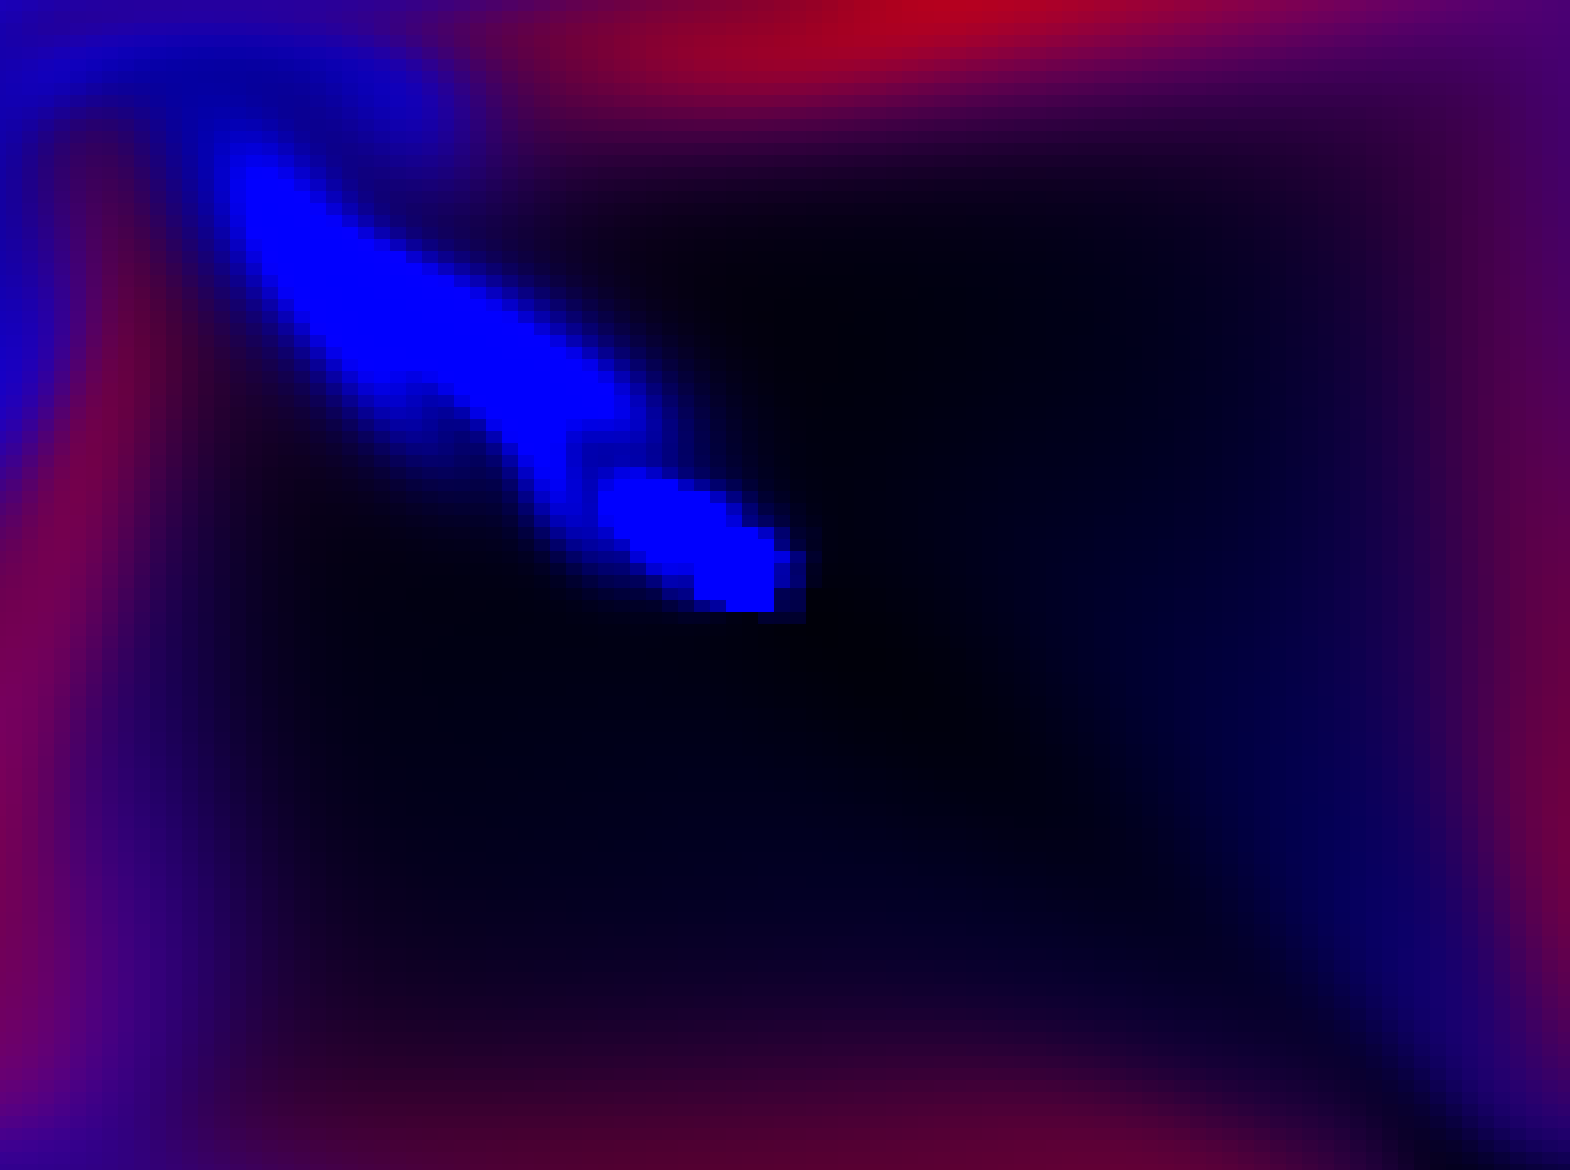
\includegraphics[width=0.45\textwidth]{../PJ_proj/bicolor.png}
    \caption{Simulation avec alternace etre le rouge et le bleu pour representer la chaleur du fluide}
\end{figure}

\satine{
    On remarque que le fluide sortant ce melange assez facilement en creant des degradés de rouge et de bleu.
}

\begin{figure}[H]
    \centering
    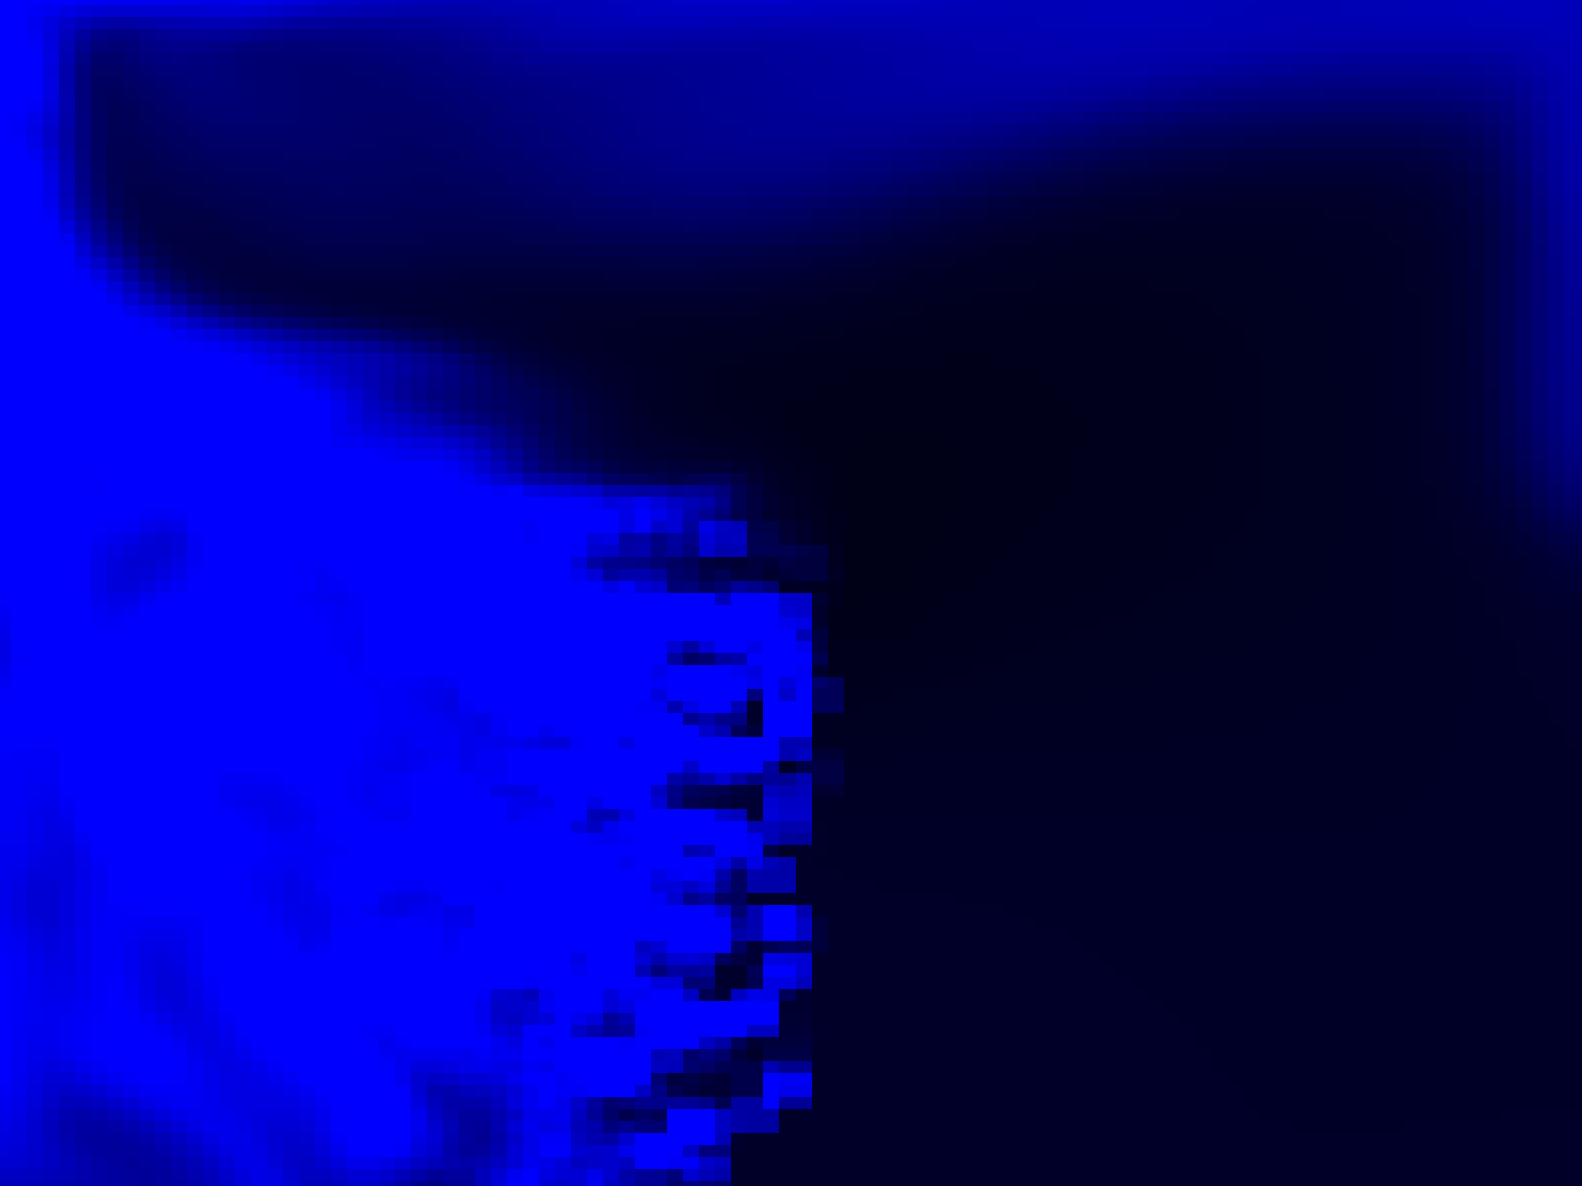
\includegraphics[width=0.45\textwidth]{../PJ_proj/line.png}
    \caption{Simulation avec sortie du fluide en ligne horizontale}
\end{figure}

\satine{
    On constate un fort fluite remplissant vite le cadre comparer au point des image au dessus.
}
\comment{}{C'est un peu mou de desccription tout ça...}
% \end{itemize}
% \end{enumerate}



\section{Gestion du Projet}
\remove{\emph{ (1-2 pages)}}
% \begin{enumerate}%pour faire une liste numérotée
%5.1    SATINE
\remove{Présenter la gestion du projet et les documents de planification rédigés (par exemple, le diagramme de Gantt).}

\subsection{Répartition des roles}

\satine{
    Durant le projet, nous avons dans un premier temps travaillé ensemble pour la mise en place de la grille de départ et la création du fluide ainsi que pour l'affichage de celui-ci. Une fois cette partie terminée, nous avons ensuite décidé de nous répartir les tâches pour être plus efficace. Ainsi, Gaelle a permis de déplacer le fluide dans diverses directions et a partir de divers points, Satine a travailler sur les obstacles, Axel à généré le code ImGui afin de pouvoir modifier les différents paramètres du fluides(densité, couleur,...) et le Bluetooth, et Saurane a travailler sur la diffusion de la chaleur.
}

\subsection{Diagramme de Gantt}

\satine{
    Nous avons réalisé un diagramme de Gantt pour planifier les différentes étapes du projet.
}
\section*{Organisation du travail - Diagramme de Gantt}
\begin{ganttchart}[
        hgrid,
        vgrid,
        time slot format=isodate,
        bar height=0.6
        ]{2024-01-01}{2024-01-14}
    \gantttitlecalendar{day} \\
    \ganttbar[bar/.style={fill=Cyan}]{\shortstack{Travail collaboratif\\creation du fluide de depart}}{2024-01-01}{2024-01-04} \\
    \ganttbar[bar/.style={fill=Cyan}]{Répartition des tâches}{2024-01-04}{2024-01-04} \\
    \ganttbar[bar/.style={fill=BrickRed}]{Creation de la diffusion chaud/froid}{2024-01-05}{2024-01-11} \\
    \ganttbar[bar/.style={fill=WildStrawberry}]{Creation des obstacles}{2024-01-05}{2024-01-11} \\
    \ganttbar[bar/.style={fill=Blue}]{Interaction avec le fluide}{2024-01-05}{2024-01-11} \\
    \ganttbar[bar/.style={fill=ForestGreen}]{Ajout de directions du fluides}{2024-01-05}{2024-01-11} \\

    \ganttbar[bar/.style={fill=Cyan}]{\shortstack{Fusion finale vers main \\+ redaction du rapport}}{2024-01-12}{2024-01-14}
\end{ganttchart}

\vspace{1cm}
\textbf{Légende :}
\begin{itemize}
  \item \textcolor{ForestGreen}{\rule{0.5cm}{0.3cm}} Gaelle
  \item \textcolor{WildStrawberry}{\rule{0.5cm}{0.3cm}} Satine
  \item \textcolor{Blue}{\rule{0.5cm}{0.3cm}} Axel
  \item \textcolor{BrickRed}{\rule{0.5cm}{0.3cm}} Saurane
  \item \textcolor{Cyan}{\rule{0.5cm}{0.3cm}} tout le monde (travail collaboratif sur la branche main)
\end{itemize}

\subsection{Branches github, commits}

\satine{
    Pour la mise en place d'un travail d'équipe optimale, nous avons utilisé GitHub. Lorsque nous travaillions ensemble, nous nous placions sur la branche main afin que chacun puisse accéder à ce que les autres ont fait facilement, puis lorsque nous avons choisi de nous repartir les taches nous nous sommes tous mis à travailler sur des branches différentes (Gaelle, Satine, Axel, Saurane) afin de pouvoir travailler et enregistrer notre travaille sans risquer de causer des conflits ou d'enregistrer quelque chose qui ne fonctionne pas. Une fois notre programme complet nous le mettions alors sur le main afin que tout le monde puisse y accéder. Nous avons également veillé à faire des commit réguliers et descriptifs pour suivre l'évolution du projet et faciliter la collaboration.
}


%5.2    SAURANE - SATINE - AXEL
\subsection{Changements majeurs effectués en cours de projet}

\begin{itemize}
  \item passage de la grille de départ à la nouvelle grille (pourquoi?)


% ============================== AXEL 6 =======================================
\axel{
 Nous avons au cours de notre projet du réadapter notre structure, en effet, nous avions préparé une grille d'essai pour tester 		notre affichage, mais lorsqu'il a fallu confronter notre prototype aux besoins du papier \emph{Stable Fluids} de Jos Stam, nous nous sommes rendu compte de besoin supplémentaires. Certains algorithmes du papier allaient avoir besoin d'échanger un certain paramètre de toutes les cellules  et notre structure ne nous le permettaient pas. Nous avons donc revu l'organisation. Nouvelles méthodes, nouveaux attributs, \emph{Setters}/  \emph{Getters} plus efficace, \emph{etc...} }

  \item la façon d'implémenter les obstacles a été modifiée quand on est passé de l'affichage d'uun obstacle à plusieurs, est-ce que ça a impacté les autres modules ? pourquoi? comment ?

\satine{
Pour la creation d'obstacle, il a fallut dans un premier temps réadapter la fonction qui délimite les bords du fluide afin que celui-ci prenne en compte les divers obstacles, ce qui a créé de nombreux problèmes (la disparition du fluide à travers l'obstacle ou la fuite du fluide à travers les bords), ou encore des problèmes de dépendance entre les différents obstacles lorsque nous avons voulu ajouter plusieurs obstacles mobiles. De plus, l'implémentation d'obstacles ayant une autre forme que la boule ( le premier obstacle programmer) pose de nombreux problèmes notamment dans la partie de délimitation du fluide ou encore dans la partie d'affichage.

Pour résoudre ces problèmes il a fallu revoir le code en changeant la façon de voir les obstacles mais également en les implémentant de manière différente. Ainsi, les obstacles ont été rangés dans une liste afin que chaque obstacle soit reconnaissable et manipulable facilement. Ils sont ainsi sélectionnés à partir de cette liste lorsqu'il faut les afficher, et c'est le dernier obstacle de la liste qui est supprimé lorsque l'on désire en retirer un. Cette organisation a également permis de mieux gérer les interactions entre plusieurs obstacles et de réduire les conflits lors de leurs déplacements.

Enfin, cette nouvelle structure a facilité l'ajout de formes différentes et leur gestion dans la simulation, en rendant le système plus flexible et plus stable dans le temps.
}   

  \item implémentation de la fenêtre pour rentrer les paramètres 

\sauranne {

Un autre changement majeur a été l'implémentation d'une fenêtre intéractive pour modifier en temps réel les paramètres de la simulation. 

Initialement, les paramètres étaient prédéfinis en dur dans le code, ce qui limitait les possibilités d'expérimentation, mais également l'accessibilité du projet pour les utilisateurs qui n'ont pas de connaissances en programmation. 
}

\end{itemize}
% \end{enumerate}


\section{Bilan et Conclusions}
\remove{Indiquer les fonctionnalités mises en œuvre par rapport au cahier des charges de départ, les points ouvertes. Les perspectives du projet décrivent ce que l'on pourrait ajouter, modifier, réécrire afin d'améliorer le projet.}
% \begin{enumerate}

%6.1     SAURANE
\subsection{Fonctionnalités rélisées présentent dans le cahier des charges}

\sauranne {
    Parmis toutes les fonctionnalités que nous avons implémentées, certaines étaient déjà prévu au moment de l'écriture du cahier des charges.
\begin{itemize}
  \item L'interface graphique composée de la fenêtre d'affichage du fluide : Cette interface graphique est bien présente dans notre projet et elle correspond presque à l'identique à ce que nous avions imaginé au départ.

  \item possibilité d'agir sur le fluide avec des curseurs : Nous avons en effet la possibilité de modofier les paramêtres du fluide en temps réel, cependant, nous avons finalement opté pour des boutons et des champs de saisie plutôt que des curseurs. Ce choix a été assez naturel car il nous permet d'étre plus précis dans le choix des paramêtres, tels que la densité ou la vitesse.
  
  \item possibilité d'ajouter des obstacles : Cette fonctionnalité a fini par être l'une des principales de notre projet, et elle permet de rendre la simulation plus ludique et plus réaliste.
\end{itemize}
}

%6.2
\subsection{Fonctionnalités non-réalisées présentent dans le cahier des charges}

\begin{itemize}
  \item possibilité de controler le fluide à distance via un smartphone (bluetooth)
  \item intégrer un mode musique qui fait réagir de fluide en focntion du son
\end{itemize}


%6.3   AXEL
\subsection{Perspectives}
\begin{itemize}
  \item Semi - lagrangien
  \item autres fonctionnalités possibles avec les obstacles, etc
\end{itemize}
% \end{enumerate}

% ============================== AXEL 7 =======================================
\axel{
Comme mentionné dans la partie \underline{\emph{\nameref{2.3 - Partie A}}}, les perspectives d'évolutions pour la suite du projet sont ces choses auxquelles nous avons songé, que nous avons essayé d'implémenter mais qui nous n'avons pas su faire aboutir. Parmi elles on peut compter :

\paragraph{Une meilleure interactivité :} Nous reprendrions l'application et le code de transmission de données et de gestion des ports afin de rendre cette fonctionnalité opérationnelle.

\paragraph{Du Semi-Lagrangien :} Nous achèverions notre implémentation du Semi-Lagrangien en intégrant la structure des particules à la mise à jour de la simulation et à l'affichage en Shader. On choisirait soit un bouton de choix entre l'Eulerien et le Semi-Lagrangien soit de superposer les deux, voir de les faire interagir, ce qui demanderait de faire des choix d'affichage en Shader et/ou de la gestion de contact.

\paragraph{Une meilleure résolution :} Nous finirions d'implémenter et d'utiliser OpenMP pour paralléliser nos calculs de mise à jour de simulation afin de se permettre d'en faire plus. En réduisant le temps de calcul, on pourrait se permettre d'augmenter le nombre de cellule tout en gardant le même nombre d'images calculées par seconde, nous permettant d'ajouter une meilleure définition à la simulation (étant actuellement de 100 cellules par 100 cellules).

}
\begin{thebibliography}{9}
\bibitem{Stam99}
Stam, J. (1999). Stable fluids. Proceedings of the 26th Annual Conference on Computer Graphics and Interactive Techniques, SIGGRAPH 1999, 121–128. https://doi.org/10.1145/311535.311548
\bibitem{Stam03}
Stam, J. (2003). Real-Time Fluid Dynamics for Games. Proceedings of the Game Developer Conference, 18(11), 17.
\bibitem{ImGUI}
https://github.com/ocornut/imgui
\bibitem{LearnOpenGL}
https://learnopengl.com/
\bibitem{heartCurve}
https://mathworld.wolfram.com/HeartCurve.html
\end{thebibliography}
\end{document}